%% Manuscript v1.0. Official MDPI template; verified v0.6/v0.7 content merged.
\documentclass[applsci,article,submit,pdftex,oneauthor]{Definitions/mdpi}
\usepackage{longtable,booktabs,array,calc,etoolbox,placeins,float}
\emergencystretch=2em
\makeatletter
\patchcmd\longtable{\par}{\if@noskipsec\mbox{}\fi\par}{}{}
\makeatother
\providecommand{\tightlist}{\setlength{\itemsep}{0pt}\setlength{\parskip}{0pt}}
\firstpage{1}
\makeatletter\setcounter{page}{\@firstpage}\makeatother
\pubvolume{1}\issuenum{1}\articlenumber{0}\pubyear{2026}\copyrightyear{2026}
\datereceived{ }\daterevised{ }\dateaccepted{ }\datepublished{ }

\Title{Risk and Coverage across Arabic Dialects in Selective Question Answering}
\newcommand{\orcidauthorA}{0000-0002-4161-2658}
\Author{Fahad AlGhamdi $^{1,*}$\orcidA{}}
\AuthorNames{Fahad AlGhamdi}
\address{$^{1}$ \quad Computer Science Department, Al-Baha University, Albaha 65779, Saudi Arabia; fghamdi@bu.edu.sa}
\corres{Correspondence: fghamdi@bu.edu.sa}

\featuredapplication{For Arabic multiple-choice question-answering systems that use confidence thresholds or prediction sets, evaluate realised risk and coverage separately for each dialect served. A target selected on Modern Standard Arabic calibration data may yield different operating points on dialectal versions of the same questions.}
\abstract{A selective-answering policy calibrated on Modern Standard Arabic (MSA) may offer different levels of service on dialectal questions. We examine this transfer on 1,420 held-out parallel questions from DialectalArabicMMLU, using four open-weight checkpoints from three model families, with AraDiCE as a second resource. An MSA threshold targeting 20\% empirical calibration risk answers fewer questions in all 20 dialect--model cells; 19 paired intervals exclude zero. Paired intervals support higher risk than MSA for Syrian in four models with calibration fixed and three under calibration resampling, and for Moroccan in two under either analysis. At the risk MSA attains when answering half the questions, Moroccan and Syrian versions are answerable on roughly a quarter to a third. At a 70\% nominal conformal-coverage target, MSA-calibrated sets lose 6--13 percentage points of coverage on these varieties; per-dialect quantiles produce sets 17--32\% larger than MSA's. The findings support joint reporting of risk and coverage by dialect. They concern multiple-choice answering, and undetected differences in meaning between the published versions may contribute to the observed gaps.}
\keyword{Arabic dialects; selective prediction; abstention; conformal prediction; calibration; large language models; distribution shift; evaluation}

% Float pagination only. Official class files, geometry, body fonts and body line spacing are unchanged.
% Avoid a separate page containing a single medium-sized figure.
\renewcommand{\topfraction}{0.95}
\renewcommand{\bottomfraction}{0.85}
\renewcommand{\textfraction}{0.05}
\renewcommand{\floatpagefraction}{0.90}
\setcounter{topnumber}{4}
\setcounter{bottomnumber}{3}
\setcounter{totalnumber}{6}
\setlength{\textfloatsep}{12pt plus 2pt minus 2pt}
\setlength{\floatsep}{10pt plus 2pt minus 2pt}
\setlength{\intextsep}{12pt plus 2pt minus 2pt}
\makeatletter
\setlength{\@fptop}{0pt}
\setlength{\@fpsep}{12pt plus 2pt minus 2pt}
\setlength{\@fpbot}{0pt plus 1fil}
\makeatother


\begin{document}

\hypertarget{introduction}{%
\section{Introduction}\label{introduction}}

A question-answering system can withhold an answer when its confidence falls below a threshold, or return a set of candidate answers calibrated to a coverage target. Choosing that policy on one language variety and using it on another raises a practical question: does the target still describe the answers users receive? We study policies chosen on labelled Modern Standard Arabic (MSA) data and applied to Egyptian, Syrian, Saudi, Emirati and Moroccan versions of the same benchmark questions.

Large language models are less accurate on dialectal Arabic than on MSA \cite{altakrori2026dialectalarabicmmlu, mousi2025aradice}, and selective prediction can widen gaps between groups \cite{jones2021selective}. Accuracy alone does not describe the service offered by an abstention policy: a system may answer fewer questions, make more errors among those it answers, or do both. We measure these outcomes when an MSA-calibrated policy is transferred to dialectal inputs, then examine how they change when calibration uses examples from the target dialect.

The evaluation uses parallel multiple-choice items and a held-out test split. In DialectalArabicMMLU \cite{altakrori2026dialectalarabicmmlu}, each question is available in MSA and five dialects through human translation. AraDiCE \cite{mousi2025aradice}, produced by machine translation and human post-editing, supplies a second resource for Egyptian and Levantine. Four open-weight checkpoints of 7--9B parameters are evaluated with a common prompt format and option-letter scoring procedure. The analysis plan and code were fixed before the confirmatory analysis; Section~\ref{pre-specification-timing-of-each-analysis-and-uncertainty} distinguishes this from specification before score collection.

An MSA threshold targeting 20\% empirical calibration risk answers fewer dialect questions in every model. Paired intervals support higher realised risk than MSA for Syrian in four models with calibration fixed and three under calibration resampling, and for Moroccan in two under either analysis. These comparisons differ from testing whether risk exceeds the nominal target. At the risk MSA attains when answering half the questions, Moroccan and Syrian versions are answerable on roughly a quarter to a third. MSA-calibrated conformal sets lose 6--13 percentage points of coverage on these varieties at a 70\% target; per-dialect quantiles produce larger sets without reaching 70\% empirical coverage in every cell. Lower confidence discrimination on Moroccan and Syrian versions and checks across four cyclic option rotations provide further context for these operating-point differences.

The contribution is a paired evaluation of policy transfer across Arabic varieties: how much of the benchmark each policy answers, the risk or set coverage it achieves, and the trade-off after per-dialect calibration. The diagnostic analyses help interpret the observed gaps, while the validity checks assess their sensitivity to potentially defective parallel items. The study releases its analysis record, code, scores and uncertainty estimates. Its conclusions concern the published question versions and the evaluated policies; Section~\ref{discussion} discusses their limits.

\hypertarget{related-work}{%
\section{Related Work}\label{related-work}}

Selective classification trades coverage for risk by allowing a classifier to abstain \cite{elyaniv2010foundations, geifman2017selective}. Its evaluation has pitfalls of its own: summaries of the risk--coverage curve such as AURC conflate accuracy with ranking quality, and Traub et al. \cite{traub2024overcoming} proposed the area under the generalised risk--coverage curve (AUGRC), an interpretable measure of undetected failures that depends on both accuracy and confidence ranking. We report both AUROC and AUGRC in Section~\ref{diagnostic-views}. Jones et al. \cite{jones2021selective} showed that abstention can widen accuracy gaps between groups, because the examples a model is unsure about are not spread evenly, and argued for group-conditional analysis. Later work studied selective classification and regression under explicit fairness constraints \cite{lee2021fair, shah2022selective}. Kamath et al. \cite{kamath2020selective} examined selective question answering under domain shift and found that softmax confidence abstains poorly out of domain. Our S4 and P1 quantities apply these ideas with dialect as the group variable and with a policy tuned on one group and used on another. Building on this work, we evaluate an MSA-calibrated policy on parallel dialectal questions and compare its operating points with those obtained after per-dialect calibration.

Split conformal prediction gives a marginal coverage guarantee under exchangeability of calibration and test data \cite{vovk2005algorithmic, angelopoulos2023conformal}. Under distribution shift, the usual guarantee need not apply, and a line of work has characterised what remains under covariate shift \cite{tibshirani2019conformal} and under more general departures \cite{barber2023conformal}. Conditional calibration within known groups (Mondrian conformal prediction) provides group-specific marginal coverage under within-group exchangeability \cite{vovk2012conditional}, and Romano et al. \cite{romano2020malice} framed equal coverage across groups as a fairness requirement. For language models, conformal methods have been applied to multiple-choice benchmarks \cite{kumar2023conformal, ye2024benchmarking}, to generation \cite{quach2024conformal, mohri2024conformal} and to settings without logit access \cite{su2024api}, and Campos et al. \cite{campos2024conformal} survey the area. Our P2 and S2 quantities measure the coverage that an MSA quantile loses on dialect inputs and the set sizes produced by per-variety quantiles at the same nominal target.

Whether language models know when they do not know has been studied through verbalised and token-level confidence \cite{kadavath2022language, xiong2024can}, through semantic uncertainty over sampled answers \cite{kuhn2023semantic}, and through selective prediction across tasks and shifts \cite{varshney2022investigating, chen2023adaptation}. Surveys of abstention in language models catalogue the policies in use and their failure modes \cite{wen2025know}. Most of this work evaluates one language. Ahuja et al. \cite{ahuja2022calibration} showed that massively multilingual models fine-tuned in English and transferred zero-shot are poorly calibrated on low-resource and typologically distant languages, and that a few labelled examples in the target language reduce the miscalibration. That work is the closest precedent for our question, at the level of language rather than dialect.

Dialect robustness has been studied as a disparity problem in English, with transformation-based parallel data \cite{ziems2022value, ziems2023multivalue} and with measurements of the dialect gap across several languages and of its economic, social and linguistic correlates \cite{kantharuban2023quantifying}. DIALECTBENCH \cite{faisal2024dialectbench} gathers evaluation sets for 281 language varieties into one benchmark, and dialect-conditioned judgements by language models have been documented as a harm in their own right \cite{hofmann2024dialect}. For Arabic, parallel dialectal corpora \cite{bouamor2018madar}, dialect-identification shared tasks \cite{abdulmageed2021nadi} and a continuous measure of dialectness \cite{keleg2023aldi} provide the linguistic background, and our similarity covariate in Section~\ref{validity-of-the-paired-versions-without-human-raters} is a coarse relative of the latter. Evaluations of Arabic-centric and general models on dialects report lower quality than on MSA \cite{huang2024acegpt, abdelali2024larabench, robinson2025alqasida}, and the two resources we use, DialectalArabicMMLU \cite{altakrori2026dialectalarabicmmlu}, which extends MMLU-Redux \cite{gema2025mmluredux, hendrycks2021mmlu}, and AraDiCE \cite{mousi2025aradice}, which translates ArabicMMLU items \cite{koto2024arabicmmlu}, were built to measure that gap. Al-Laith and Kebdani \cite{allaith2025calibration} evaluated the calibration of eight pre-trained models on Arabic dialect identification and found that it varies across dialects, but their object is the confidence of the dialect classifier, whereas ours is the transfer of an answer policy across parallel phrasings. A published quality screen of DialectalArabicMMLU \cite{ifm2026verified} removes rows that three LLM judges flag unanimously, and we use it as an external filter.

The measurement we rely on, scoring option letters by next-token probability \cite{robinson2023leveraging}, has known weaknesses. Surface-form competition can split probability mass among equivalent strings \cite{holtzman2021surface}; option order and option labels bias the choice \cite{zheng2024robust, pezeshkpour2024sensitivity, alzahrani2024benchmarks}; first-token probabilities and generated text can disagree, mostly for instruction-tuned models \cite{wang2024myanswer, lyu2024beyond}; and some benchmark items can be answered without their question \cite{balepur2024artifacts}. Translated benchmarks add a second layer of doubt: translation artefacts affect cross-lingual comparisons \cite{artetxe2020translation}, and translated MMLU variants carry errors and culturally mismatched items \cite{singh2024global}. Language-model judges, which we use in a screening role, have documented biases of their own \cite{zheng2023judging, chiang2023can}. Sections 4.2 and 4.4 address the parts of this that we could test, with four cyclic rotations, free and chat-template generation, an external filter, a similarity covariate, a second resource and a model-assisted screen whose limits are stated where it is used.

\hypertarget{materials-and-methods}{%
\section{Materials and Methods}\label{materials-and-methods}}

\hypertarget{resources}{%
\subsection{Resources}\label{resources}}

DialectalArabicMMLU (DAMM) \cite{altakrori2026dialectalarabicmmlu} contains 3,135 four-option questions drawn from MMLU-Redux, each available in MSA, Egyptian (EGY), Syrian (SYR), Saudi (KSA), Emirati (UAE), Moroccan (MAG) and English. The dialect versions were produced by manual translation and adaptation through a language-service provider, with a translator, a reviewer and an adjudicator per dialect. The resource's authors report a quality check of 32 items per dialect in which about 5\% of translations contained inaccuracies, and a second review round for the Emirati and Syrian sets. A shared key identifies a question across varieties. We keep the resource's label MAG for the Moroccan set.

AraDiCE \cite{mousi2025aradice} serves as a second resource. Its ArabicMMLU items \cite{koto2024arabicmmlu} were machine-translated into Egyptian and Levantine (LEV) and human post-edited, and they are paired with the ArabicMMLU MSA originals. We sampled 2,000 parallel items (600 for calibration, 1,400 for test, stratified by subject group). AraDiCE has no Moroccan variety, so the Moroccan results rest on DAMM alone.

\hypertarget{models}{%
\subsection{Models}\label{models}}

We evaluate ALLaM-7B-Instruct-preview \cite{bari2025allam}, Fanar-1-9B \cite{fanar2025}, Qwen3-8B-Base \cite{qwen3} and gemma-2-9b \cite{gemma2}, all open weights, run locally in bf16. ALLaM is the only instruction-tuned checkpoint, the other three being base models. Fanar-1-9B is a continual pre-training of the Gemma-2-9B base model \cite{fanar2025}, so the four checkpoints come from three base families. We report them as four models because their outputs differ materially, and we return to the shared base in Section~\ref{discussion}.

\hypertarget{measurement}{%
\subsection{Measurement}\label{measurement}}

Arabic-variety prompts contain an Arabic instruction, three fixed MSA demonstrations, and the question with four options labelled A to D. English prompts use an English instruction and English demonstrations. For each letter, the scorer collects unique token identifiers for its space-prefixed and unprefixed forms when each is a single token; if neither is, it uses the final token of the space-prefixed form. Their log-probabilities are combined by log-sum-exp and renormalised over the four letters. The answer is the highest-scoring letter, confidence is its renormalised probability $p_{\max}$, and conformal nonconformity is $1-p_{\mathrm{true}}$. Models ran locally in bf16 on Apple-silicon MPS, in evaluation mode, with left padding, a maximum input length of 2,048 tokens and batches sorted by prompt character length. The checkpoints were loaded by name without pinned revisions; exact weight revisions and the complete original dependency lock were not recorded. Original-order re-scoring and raw-prompt generation reuse the main prompt. Rotation checks change option order, and the separate ALLaM check uses its chat template (Section~\ref{robustness-of-the-measurement}). Stored option log-probabilities have four decimals and derived probabilities five; Appendix~\ref{independent-computational-check} describes the resulting boundary effects.

\hypertarget{splits}{%
\subsection{Splits}\label{splits}}

A domain-stratified development sample of 500 keys (seed 0) was used to design the study and is reported only as development. Three further keys supplied the fixed demonstrations and were excluded from the confirmatory pool (3,135 -- 500 -- 3 = 2,632). The remaining 2,632 keys were allocated before confirmatory scoring began (seed 20261105) to router training (404 keys), calibration (808) and test (1,420), with all varieties of a key kept in the same split. All primary estimates are computed on the test keys and every deployable threshold or quantile is chosen on the calibration keys. The one quantity that reads test labels to choose its operating point is P1, which is descriptive by design (Section~\ref{quantities}). The seeds 20261104 and 20261106 belong to the samples drawn for the equivalence screen (Section~\ref{validity-of-the-paired-versions-without-human-raters}), not to the splits.

\hypertarget{pre-specification-timing-of-each-analysis-and-uncertainty}{%
\subsection{Pre-specification, timing of each analysis, and uncertainty}\label{pre-specification-timing-of-each-analysis-and-uncertainty}}

The local project record distinguishes specification before scoring from specification before analysis. Splits and scoring scripts were fixed on 4 November before scoring began at 20:57. The first analysis plan and code, covering P1--P3 and S1--S3, were recorded at approximately 21:30 during ALLaM scoring; S4 was added at approximately 23:30 during Qwen3 scoring. The record states that no confirmatory score file had been opened for analysis at either point. The confirmatory analysis ran the next morning. Later analyses were specified in dated addenda after the main results had been seen and before their own computation, except for the post-hoc summaries identified in Table~\ref{tab:1}. This was a locally documented plan rather than a public pre-registration \cite{nosek2018preregistration, vanmiltenburg2021preregistering}. Appendix~\ref{plan-history-and-freeze-log} records the chronology and a timestamp inconsistency. File hashes identify the archived code but do not independently establish when it existed.

\begin{table}[!htbp]\footnotesize\setlength{\tabcolsep}{4pt}
\caption{Analyses by the time of their specification.}\label{tab:1}
\begin{tabular}{@{}
  >{\raggedright\arraybackslash}p{(\columnwidth - 4\tabcolsep) * \real{0.2581}}
  >{\raggedright\arraybackslash}p{(\columnwidth - 4\tabcolsep) * \real{0.3548}}
  >{\raggedright\arraybackslash}p{(\columnwidth - 4\tabcolsep) * \real{0.3871}}@{}}
\toprule\noalign{}
\begin{minipage}[b]{\linewidth}\raggedright
Tier
\end{minipage} & \begin{minipage}[b]{\linewidth}\raggedright
Analyses
\end{minipage} & \begin{minipage}[b]{\linewidth}\raggedright
Specified
\end{minipage} \\
\midrule\noalign{}
Specified before the confirmatory analysis & P1, P2, P3, S1, S2, S3 & plan v1 and code v1 written during score collection (ALLaM about half scored), code frozen by sha256; no score file had been read \\
Specified before the confirmatory analysis, added during collection & S4 & added to the frozen code with ALLaM complete and Qwen3 partly scored; no confirmatory file opened for analysis \\
Addendum, before its computation & screen sensitivity analyses & after the main results; frozen before computation \\
Addendum, before its computation & validity layers L1, L2, L4 & same \\
Addendum, before its computation & diagnostic views (accuracy, discrimination, D4) & same \\
Addendum, before its computation & robustness protocol (rotations, generation, re-scoring) & before the robustness scoring \\
Addendum, before its computation & verification package (double resampling, paired rotation comparison, independent check) & same \\
Addendum, before its computation & risk-difference and generated-answer supplements & same \\
Exploratory / post hoc & ceiling counts for D4 (Section~\ref{diagnostic-views}) & after the relevant results were seen \\
Claim withdrawn & P3 as a stand-alone measure of dialect-specific instability & after the robustness protocol (Section~\ref{robustness-of-the-measurement}) \\
\bottomrule\noalign{}
\end{tabular}
\end{table}

Uncertainty is quantified by a paired percentile bootstrap over test keys \cite{efron1993bootstrap, koehn2004statistical}, with 2,000 replicates and 95\% intervals while calibration is held fixed. A sensitivity analysis independently resamples calibration and test keys, preserving pairing across varieties and re-selecting thresholds or quantiles in each of 1,000 replicates. Both intervals are reported for quantities materially affected by calibration uncertainty. Point estimates are observed-sample values and differences. Intervals are pointwise, without multiplicity adjustment; counts of intervals excluding a reference value describe the observed pattern rather than simultaneous confidence across all cells. Following cautions about significance testing in NLP \cite{dror2018hitchhiker}, we report effect sizes with intervals. Appendix~\ref{independent-computational-check} explains the distinction between sample differences and bootstrap-mean centres.

\hypertarget{quantities}{%
\subsection{Quantities}\label{quantities}}

Every quantity compares a variety v with MSA on the same test keys. They answer different questions and should not be read as substitutes for one another.

S4, operational selective prediction, is the primary operational evidence for the transferred abstention policy. On MSA calibration items, we sort by confidence and compute the error rate $r_k$ among the $k$ most confident. The threshold $\tau$ is the confidence at the end of the largest prefix satisfying $r_k \leq r^*$; if none qualifies, $\tau=1.01$. Test items are accepted when their confidence is at least $\tau$, using the same threshold for every variety. This includes all items tied at the boundary, so the threshold rule can accept more items than the qualifying prefix (Appendix~\ref{independent-computational-check}). We report answered fraction, realised risk among accepted items and paired differences from MSA at $r^*\in\{0.15,0.20,0.25,0.30\}$, with 0.20 as the main target. The target is an empirical calibration-risk ceiling; it supplies no finite-sample guarantee for test risk.

P1, the answerable fraction at the MSA-matched risk, is descriptive. Let t be the risk MSA attains on test when it answers its 50\% most confident questions. For each variety, P1 is the largest fraction of questions that can be answered, in confidence order, while keeping the error rate at or below t. Because the largest qualifying prefix can extend a little beyond the half-way point, MSA's own P1 is approximately rather than exactly 0.50 (0.5000$-$0.5014 across the four models), and the differences are taken from these actual values. P1 reads the risk from test labels and uses an oracle threshold. It describes the risk--coverage curves, is not a deployable policy, and has an operating point different from S4's.

P2 concerns split-conformal prediction sets. With nonconformity $1-p_{\mathrm{true}}$, we take the calibration order statistic at rank $\lceil(n+1)(1-\alpha)\rceil$ as the quantile $\hat q$. A prediction set contains each option whose nonconformity is at most $\hat q$. We measure test coverage under the MSA quantile and mean set size under each variety's own quantile, including the ratio to MSA's set size at the same nominal target. The usual marginal coverage guarantee assumes exchangeable calibration and test examples, an assumption that cannot be taken for granted when transferring from MSA to dialect inputs. The main error level is $\alpha=0.30$, with $\alpha=0.10$ also reported.

S2 compares four calibration policies for dialect inputs with an equal number of calibration keys per variety: a pooled calibration set, group-conditional (Mondrian) calibration with the true variety label, the same with a variety predicted by a character n-gram classifier trained on the router split, and a conservative rule that unions the sets of the varieties the classifier considers plausible. We report achieved coverage and set size, and the fraction of the oracle's coverage gain that each practical method recovers. Equal keys per variety is not equal annotation: the MSA-only quantile uses 808 calibration rows, whereas the pooled set uses 808 $\times$ 7 variety rows and each Mondrian group its own 808, and the classifier is trained on 404 $\times$ 7 texts. A policy that predicts the variety carries no coverage guarantee for the true variety.

D4 re-selects the S4 threshold on the calibration items of each variety (same rule, same target) and evaluates it on that variety's test items: realised risk, answered fraction, the contrast with the transferred threshold, and the residual gap to MSA at the same nominal target.

Confidence discrimination is measured by the AUROC of $p_{\max}$ for correct versus incorrect answers. We also report AUGRC \cite{traub2024overcoming}, which reflects both accuracy and confidence ranking, with comparisons paired by key. The robustness analyses examine option-order sensitivity across four cyclic rotations, stability of the gaps over those rotations, agreement between generated and letter-logit answers, and re-run reproducibility.

None of these quantities amounts to a guarantee for dialect users: S4 targets an empirical risk on a calibration sample, the conformal guarantee is marginal and depends on exchangeability, and equalising a nominal target does not equalise achieved risk. For that reason realised risk and achieved coverage are always shown next to the policy's output.

\hypertarget{use-of-generative-ai-tools}{%
\subsection{Use of generative AI tools}\label{use-of-generative-ai-tools}}

Claude Fable 5.1 (Anthropic; \nolinkurl{claude-fable-5-1}), accessed through Claude Code during 4--8 November 2026, was used to write and revise analysis and plotting code, run local model-scoring workflows, maintain the claims ledger, and draft and revise the manuscript. This identifier was recorded for the manuscript-preparation sessions; model versions for earlier sessions were not consistently logged. OpenAI tools, including ChatGPT and Codex, were used to review analysis plans, code and drafts. GPT-6 Astra is recorded for some review sessions; exact versions were not retained for every session. A Codex-assisted comparison of displayed estimates with result files identified the reporting correction documented in Appendix~\ref{independent-computational-check}. The author reviewed and edited this work and is responsible for the design, analyses, interpretations and final manuscript.

LLM judgments also enter the validity analyses. L1 uses a published filter based on three LLM judges \cite{ifm2026verified}; the translation-equivalence screen used separate GPT-6 Astra Extra High sessions for two ratings and adjudication. Section~\ref{validity-of-the-paired-versions-without-human-raters} and Appendix~\ref{model-assisted-screen} describe these screens and their uncertainty. They provide automated screening evidence, with no human equivalence assessment.

\hypertarget{results}{%
\section{Results}\label{results}}

Models are given in the order ALLaM, Fanar, Qwen3 and Gemma throughout; their MSA accuracies are 0.59, 0.61, 0.63 and 0.59. The held-out test follows the pattern observed in development, with narrower intervals. A separate implementation reproduced P1 exactly and closely reproduced the main S4 and P2 results; Appendix~\ref{independent-computational-check} reports the boundary differences and the scope of this check.

\hypertarget{confirmatory-results-1420-held-out-questions}{%
\subsection{Confirmatory results (1,420 held-out questions)}\label{confirmatory-results-1420-held-out-questions}}

Under the MSA-calibrated threshold for a 20\% target (S4; Figure~\ref{fig:s4}), MSA users receive an answer on 0.52 / 0.56 / 0.59 / 0.47 of the questions at a realised risk of 0.21 / 0.19 / 0.20 / 0.18. Table~\ref{tab:2} gives the dialect users' side.

\begin{table}[!htbp]\footnotesize\setlength{\tabcolsep}{4pt}
\caption{S4 at the MSA-calibrated threshold (target 0.20): paired differences in answered fraction, realised risk for the dialect user, and the cells in which the paired risk difference against MSA excludes zero (fixed-calibration bootstrap). Within each numeric cell, the first line gives ALLaM / Fanar and the second Qwen3 / Gemma. Risk differences in the final column are in percentage points.}\label{tab:2}
\begin{tabular}{@{}
  >{\raggedright\arraybackslash}p{(\columnwidth - 6\tabcolsep) * \real{0.0698}}
  >{\raggedright\arraybackslash}p{(\columnwidth - 6\tabcolsep) * \real{0.2791}}
  >{\raggedright\arraybackslash}p{(\columnwidth - 6\tabcolsep) * \real{0.2791}}
  >{\raggedright\arraybackslash}p{(\columnwidth - 6\tabcolsep) * \real{0.3721}}@{}}
\toprule\noalign{}
\begin{minipage}[b]{\linewidth}\raggedright
Var.
\end{minipage} & \begin{minipage}[b]{\linewidth}\raggedright
$\Delta$ answered fraction vs MSA
\end{minipage} & \begin{minipage}[b]{\linewidth}\raggedright
realised risk for the dialect user
\end{minipage} & \begin{minipage}[b]{\linewidth}\raggedright
$\Delta$ risk vs MSA with CI excluding 0
\end{minipage} \\
\midrule\noalign{}
MAG & \begin{tabular}[t]{@{}l@{}}$-$0.11 / $-$0.15\\$-$0.21 / $-$0.18\end{tabular} & \begin{tabular}[t]{@{}l@{}}0.28 / 0.21\\0.24 / 0.17\end{tabular} & ALLaM +6.7 {[}+3.1, +10.1{]}; Qwen3 +3.5 {[}+0.3, +7.0{]}; not Fanar, not Gemma (2/4) \\
SYR & \begin{tabular}[t]{@{}l@{}}$-$0.05 / $-$0.13\\$-$0.12 / $-$0.12\end{tabular} & \begin{tabular}[t]{@{}l@{}}0.31 / 0.23\\0.23 / 0.22\end{tabular} & +9.3 / +3.7 / +3.1 / +4.2 points (4/4) \\
EGY & \begin{tabular}[t]{@{}l@{}}$-$0.04 / $-$0.08\\$-$0.06 / $-$0.07\end{tabular} & \begin{tabular}[t]{@{}l@{}}0.25 / 0.21\\0.22 / 0.22\end{tabular} & ALLaM, Gemma (2/4) \\
KSA & \begin{tabular}[t]{@{}l@{}}$-$0.05 / $-$0.07\\$-$0.07 / $-$0.07\end{tabular} & \begin{tabular}[t]{@{}l@{}}0.24 / 0.22\\0.20 / 0.21\end{tabular} & Gemma (1/4) \\
UAE & \begin{tabular}[t]{@{}l@{}}$-$0.01 / $-$0.05\\$-$0.05 / $-$0.03\end{tabular} & \begin{tabular}[t]{@{}l@{}}0.26 / 0.20\\0.21 / 0.19\end{tabular} & ALLaM (1/4) \\
\bottomrule\noalign{}
\end{tabular}
\end{table}

The answered-fraction difference excludes 0 in 19 of 20 cells (all but ALLaM--UAE), with or without calibration resampling. The paired risk difference against MSA excludes 0 for Syrian in four models (three under calibration resampling, where Gemma's interval comes to include 0) and for Moroccan in two (ALLaM and Qwen3, both ways). Only in those cells do we speak of a ``double penalty'', meaning fewer answers and a higher error rate than MSA. Whether the 20\% target itself is exceeded is a separate question. Point estimates lie above 0.20 in 18 of 20 dialect cells (Qwen3--Saudi by 0.0003), but with the fixed-calibration interval only ALLaM's five dialects exceed it with confidence (0.24$-$0.31), and under calibration resampling only ALLaM--Moroccan and ALLaM--Syrian do. MSA's own realised risk is 0.213 for ALLaM and 0.200 for Qwen3, a reminder that the rule targets an empirical risk on 808 calibration items and that the test realisation can sit above the target for MSA as well.

\begin{figure}[!htbp]
\centering
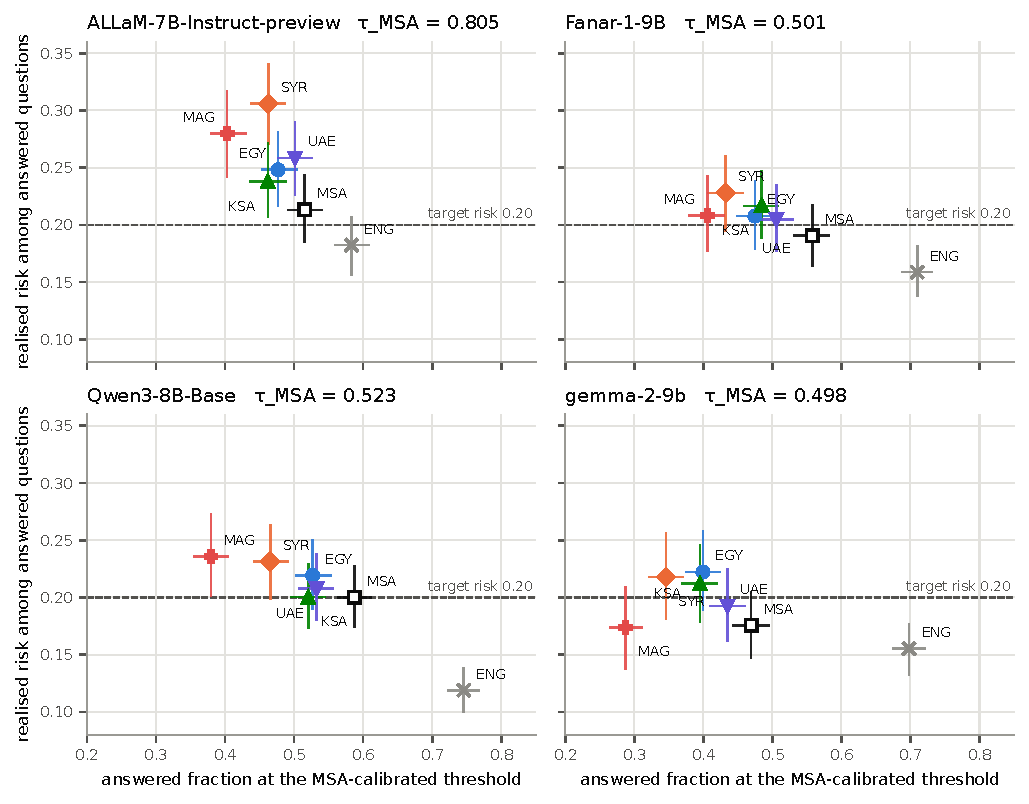
\includegraphics[width=\textwidth,height=0.43\textheight,keepaspectratio]{figures/fig1_s4_transfer.pdf}
\caption{S4: an abstention threshold chosen on MSA calibration data for a 20\% target risk, applied unchanged to every variety (1,420 test keys). Each point is one variety's answered fraction and realised risk, with 95\% key-bootstrap intervals (threshold fixed); the hollow square is MSA and the dashed line the target. $\tau_{\mathrm{MSA}}$ is given per model.}
\label{fig:s4}
\end{figure}

At the risk attained by MSA when answering half the questions (P1; Table~\ref{tab:p1full} and Figures~\ref{fig:p1} and~\ref{fig:curves}), the Moroccan versions are answerable on 0.23$-$0.32 of the questions across the four models ($\Delta$ $-$0.18 to $-$0.27), the Syrian on 0.31$-$0.34 ($\Delta$ $-$0.16 to $-$0.19), the Egyptian on 0.35$-$0.41 ($-$0.09 to $-$0.15), the Saudi on 0.37$-$0.44 ($-$0.06 to $-$0.13) and the Emirati on 0.42$-$0.44 ($-$0.06 to $-$0.08). All 20 intervals exclude 0. Since P1 and S4 are different operating points, the two sets of differences are not directly comparable.

For conformal sets at $\alpha$ = 0.30 (P2; Figure~\ref{fig:p2} and Table~\ref{tab:p2coverage}), coverage under the MSA quantile falls by 8$-$13 points for MAG and by 6$-$9 points for SYR, with the other dialects losing 3$-$5 points. A per-variety quantile at the same nominal target produced sets $\times$1.17$-$1.32 for MAG, $\times$1.18$-$1.23 for SYR and $\times$1.08$-$1.17 for the Gulf varieties. The double-resampled intervals for these ratios are 2.7$-$4.3 times wider than the fixed-calibration ones and still exclude 1 in all 20 cells, although the target was not met empirically in every cell (Table~\ref{tab:p2coverage}). At $\alpha$ = 0.10 the coverage differences are at most 1.7 points and 19 of 20 intervals include 0, so the phenomenon belongs to the operating range we studied rather than to every target.

\begin{figure}[!htbp]
\centering
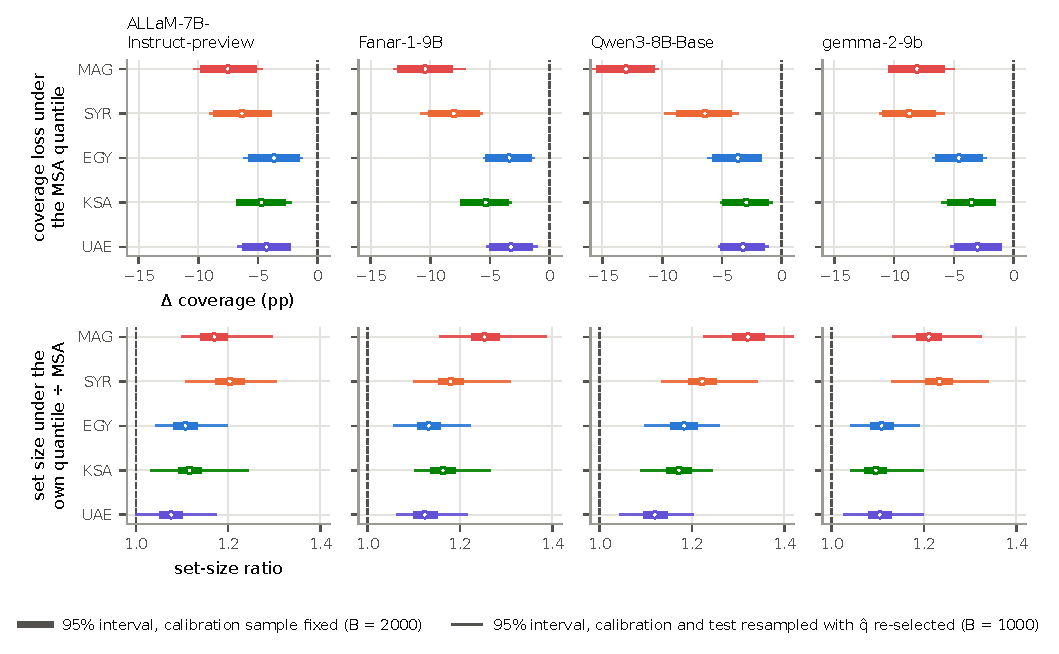
\includegraphics[width=\textwidth,height=0.43\textheight,keepaspectratio]{figures/fig3_p2_conformal.pdf}
\caption{P2: split-conformal sets at $\alpha$ = 0.30 (nominal coverage 0.70). Top: coverage lost on each dialect under the MSA quantile. Bottom: the set size each dialect's own quantile produced at the same nominal target, relative to MSA. Thick bars: 95\% intervals with the calibration sample fixed; thin bars: calibration and test keys resampled with the quantile re-selected.}
\label{fig:p2}
\end{figure}

Variety-aware calibration (S2; $\alpha$ = 0.30, MAG, target 0.70, equal calibration keys per variety; Table~\ref{tab:s2full}) raises coverage from 0.57$-$0.62 under the MSA quantile to 0.62$-$0.65 with a pooled calibration set, to 0.63$-$0.68 with a character n-gram variety classifier, and to 0.66$-$0.69 with the true variety label (Mondrian), while the mean set size grows from 1.14$-$1.44 to 1.53$-$1.72. The text classifier recovers 51$-$88\% of the oracle's gain, least in ALLaM and most in Gemma. ALLaM--MAG stays below the target even with the true label (0.657). Calibration-sample variability remains a possible explanation, which this analysis does not establish.

AraDiCE also shows lower accuracy, answerable fraction and transferred-set coverage for Egyptian and Levantine than for MSA (Section~\ref{validity-of-the-paired-versions-without-human-raters}).

\hypertarget{validity-of-the-paired-versions-without-human-raters}{%
\subsection{Validity of the parallel items}\label{validity-of-the-paired-versions-without-human-raters}}

The comparisons above assume that a dialect version asks the same question as its MSA original. We assessed this assumption using an LLM-based equivalence screen and complementary sensitivity analyses; no human equivalence ratings were available.

In a model-assisted screen, 400 pairs (80 keys $\times$ 5 dialects, of which 50 development and 30 test keys; 150 double-rated) were judged by GPT-6 Astra Extra High in two separate sessions, with a third session as adjudicator (Appendix~\ref{model-assisted-screen}). The screen's basic flag is a negative judgement on either meaning preservation (a changed condition, quantity or term) or the validity of the answer and options. This composite flag was raised on 0.37 {[}0.31, 0.43{]} of the pairs (UAE 0.44, EGY 0.33). The answer or options were judged invalid on 0.08 (MAG 0.16), and a hint or an ambiguity was judged to have been added on 0.34. Because the answer-validity judgement was ``unsure'' on 29\% of pairs, the complement of the 0.08 is not a confirmed-valid rate. Agreement between the two sessions was $\kappa$ = 0.86 for meaning, 0.36 for answer validity (mostly ``yes'' against ``unsure'') and 0.90 for clarity \cite{cohen1960kappa}. These figures measure the consistency of one model with itself and are not inter-annotator agreement. The screen's criteria and sampling frame differ from the resource authors' 32-item check. Its flag rates are therefore not directly comparable with that check and do not estimate the resource's error rate.

Whether the flags fall where the models fail could not be settled on this sample. On 1,600 pair $\times$ model observations, accuracy dropped by 4.5 points on unflagged pairs and by 6.2 on flagged ones (difference $-$1.8 {[}$-$8.2, +5.1{]}), and the answer changed in 26.9\% against 27.7\%. The two are not detectably different, but the interval is wide enough to allow a material association. After excluding flagged pairs on the 80 audited keys, answered-fraction differences averaged across models remained negative ($-$6 to $-$20 percentage points). P1 estimates were much less precise; Moroccan interval widths ranged from 38 to 94 points. The worst-case bound for fixed-rule proportions, $f/(1-f)$, is uninformative at these flag rates.

Three automatic layers were specified after the main results and before their computation (Addendum 4). The first (L1) is the external filter. Its screening pool was selected from items that strong baselines answered wrongly rather than from a random sample. Of the 935 dialect rows that three LLM judges flag unanimously in the resource \cite{ifm2026verified}, 387 fall on test keys (5$-$6\% per dialect). Dropping each flagged key from the dialect and from its paired MSA comparison changes every endpoint by at most 1.5 points ($\Delta$P1, ALLaM--Syrian), and most by less than one point, in all 20 dialect $\times$ model cells. The second (L2) is a similarity covariate. The cost varies with embedding similarity to the MSA text (multilingual-e5-large \cite{wang2024multilinguale5}) in every cell, and the most similar tercile retains at least two thirds of the full-sample P1 gap in three of four models for SYR and EGY, and in two or three for MAG depending on row-order tie breaking; KSA and UAE meet that cutoff in at most one model. The pattern is descriptive, since similarity may reflect both linguistic differences and item difficulty. The third (L4) is the second resource. On AraDiCE (1,400 test items; machine translation with human post-editing) accuracy drops by 3.6$-$7.0 points, the MSA-matched answerable fraction by 11$-$17 points for EGY and 6$-$14 for LEV, and coverage under the MSA quantile by 3$-$7 points, with intervals below zero in all eight cells for accuracy, answerable fraction and coverage, and set sizes grow $\times$1.02$-$1.28 (point estimates; no interval was computed for the ratios in this layer). The recurrence of these gaps under a different translation pipeline speaks against translation artefacts as the whole explanation, but it cannot exclude artefacts shared by both pipelines, and it says nothing about Moroccan, which AraDiCE does not cover.

The gaps persisted across the two resources and the specified automatic sensitivity analyses. These checks reduce reliance on any one translation pipeline or filter, but undetected meaning differences may still contribute to the measured gaps. The available human validity evidence comes from the resources' translation and post-editing procedures.

\hypertarget{diagnostic-views}{%
\subsection{Diagnostic views}\label{diagnostic-views}}

The views in this section were specified after the confirmatory results and before they were computed (Table~\ref{tab:1}). They describe the same 1,420 test keys from three angles and are not additive components, so we do not attribute a share of the gap to any one of them.

Dialect accuracy is lower in every cell (Table~\ref{tab:accuracyfull}): against 0.59$-$0.63 on MSA, the models reach 0.49$-$0.53 on Moroccan and 0.50$-$0.58 on Syrian versions.

Choosing the S4 threshold on each variety's own calibration items instead of MSA's, with the same rule and the same target of 0.20, and applying it to that variety's test items gives a realised risk of 0.16$-$0.24 across the 20 cells (against 0.17$-$0.31 under the transferred MSA threshold), while reducing the answered fraction in 17 of 20 cells, with intervals below zero for those contrasts (Figure~\ref{fig:d4}). The other three cells have higher answered fractions after re-selection (Fanar--EGY, Gemma--KSA and Gemma--UAE). The residual gap to MSA at the same nominal target is $-$0.01 to $-$0.34, with CI \textless{} 0 in 19 of 20 cells when the calibration sample is held fixed and in 14 of 20 under double resampling (Section~\ref{robustness-of-the-measurement}). As a post-hoc descriptive summary, we count cells above the target ceiling rather than measuring their distance from it. Under the transferred threshold the realised risk lies above 0.20 in 18 of 20 dialect cells (point estimates) and above 0.24 in four, all of them ALLaM. Under the re-selected threshold it lies above 0.20 in 7 cells and above 0.24 in none. Where the transferred threshold was already near the ceiling, re-selection mostly traded answers for small changes in risk (Qwen3--EGY, for instance: risk 0.22 $\rightarrow$ 0.17, answered 0.53 $\rightarrow$ 0.42). The realised risks under $\tau_v$ happen to fall within $\pm$0.04 of 0.20, but that is the observed range, not a tolerance or a guarantee.

\begin{figure}[!htbp]
\centering
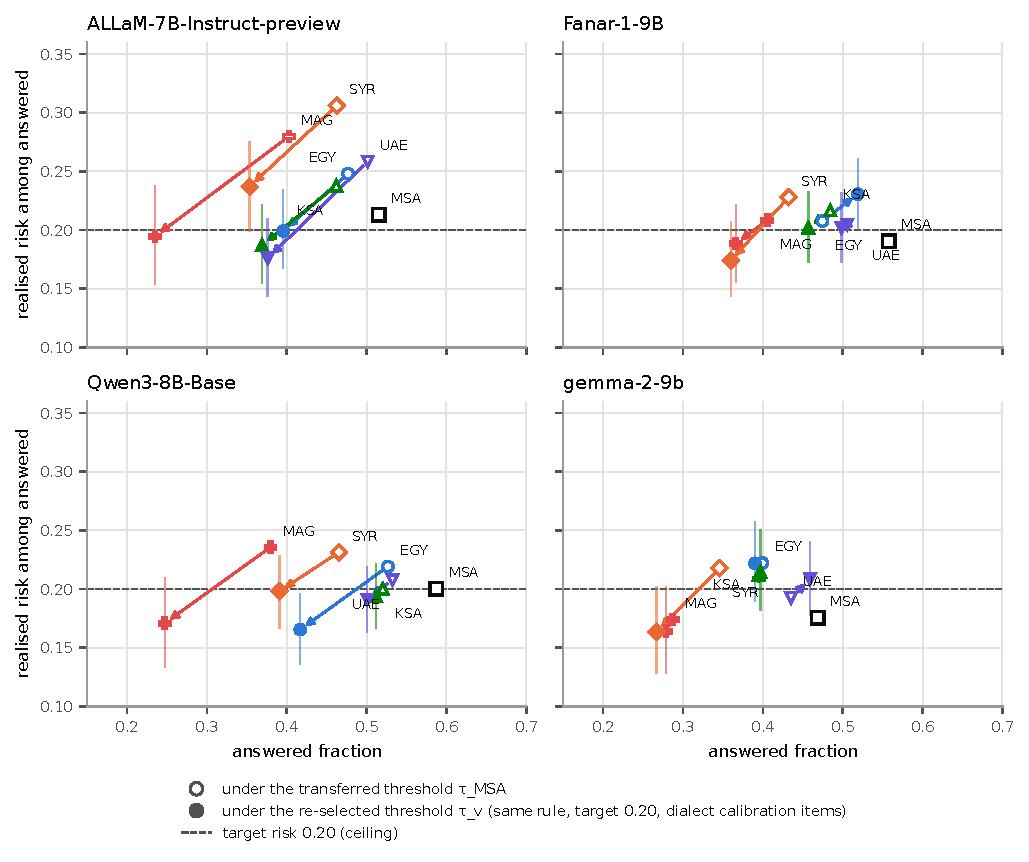
\includegraphics[width=\textwidth,height=0.43\textheight,keepaspectratio]{figures/fig2_d4_adaptation.pdf}
\caption{D4: re-selecting the threshold on each dialect's own calibration items (same rule, same target). Each arrow runs from the operating point under the transferred MSA threshold (hollow marker) to the one under the re-selected threshold (filled); vertical bars are the 95\% interval of the realised risk at $\tau_v$; the hollow square is MSA under its own threshold.}
\label{fig:d4}
\end{figure}

\begin{table}[!htbp]\footnotesize\setlength{\tabcolsep}{4pt}
\caption{$\Delta$AUROC (variety -- MSA), $p_{\max}$ as the score, paired by key, with 95\% intervals.}\label{tab:3}
\begin{tabular}{@{}
  >{\raggedright\arraybackslash}p{(\columnwidth - 10\tabcolsep) * \real{0.0769}}
  >{\raggedright\arraybackslash}p{(\columnwidth - 10\tabcolsep) * \real{0.2051}}
  >{\raggedright\arraybackslash}p{(\columnwidth - 10\tabcolsep) * \real{0.2051}}
  >{\raggedright\arraybackslash}p{(\columnwidth - 10\tabcolsep) * \real{0.2051}}
  >{\raggedright\arraybackslash}p{(\columnwidth - 10\tabcolsep) * \real{0.2051}}
  >{\raggedright\arraybackslash}p{(\columnwidth - 10\tabcolsep) * \real{0.1026}}@{}}
\toprule\noalign{}
\begin{minipage}[b]{\linewidth}\raggedright
\end{minipage} & \begin{minipage}[b]{\linewidth}\raggedright
ALLaM
\end{minipage} & \begin{minipage}[b]{\linewidth}\raggedright
Fanar
\end{minipage} & \begin{minipage}[b]{\linewidth}\raggedright
Qwen3
\end{minipage} & \begin{minipage}[b]{\linewidth}\raggedright
Gemma
\end{minipage} & \begin{minipage}[b]{\linewidth}\raggedright
CIs excluding 0
\end{minipage} \\
\midrule\noalign{}
MAG & $-$0.045 {[}$-$.072, $-$.015{]} & $-$0.040 {[}$-$.063, $-$.014{]} & $-$0.059 {[}$-$.087, $-$.032{]} & $-$0.029 {[}$-$.057, $-$.001{]} & 4/4 \\
SYR & $-$0.056 {[}$-$.084, $-$.028{]} & $-$0.038 {[}$-$.063, $-$.012{]} & $-$0.065 {[}$-$.091, $-$.039{]} & $-$0.036 {[}$-$.063, $-$.009{]} & 4/4 \\
EGY & $-$0.023 {[}$-$.050, +.002{]} & $-$0.037 {[}$-$.060, $-$.015{]} & $-$0.031 {[}$-$.055, $-$.008{]} & $-$0.020 {[}$-$.044, +.005{]} & 2/4 \\
KSA & $-$0.012 {[}$-$.037, +.011{]} & $-$0.033 {[}$-$.057, $-$.010{]} & $-$0.015 {[}$-$.037, +.006{]} & $-$0.027 {[}$-$.050, $-$.004{]} & 2/4 \\
UAE & +0.002 {[}$-$.022, +.026{]} & $-$0.013 {[}$-$.035, +.010{]} & $-$0.014 {[}$-$.039, +.009{]} & $-$0.005 {[}$-$.028, +.018{]} & 0/4 \\
\bottomrule\noalign{}
\end{tabular}
\end{table}

MSA AUROC is 0.77$-$0.80. On Moroccan and Syrian versions the confidence score separates correct from incorrect answers less well in all four models, on Egyptian and Saudi in two of four, and on Emirati the difference is not detectable on this sample (Table~\ref{tab:3}). AUGRC \cite{traub2024overcoming}, which combines accuracy and ranking, is worse than MSA in all 20 cells. These differences are subject to the same questions of pair and label validity as everything else (Section~\ref{validity-of-the-paired-versions-without-human-raters}), and they do not show that every threshold, or a different confidence score, would fail.

\hypertarget{robustness-of-the-measurement}{%
\subsection{Robustness of the measurement}\label{robustness-of-the-measurement}}

The robustness protocol was specified before the robustness scoring for option order and answer extraction, and before computation for calibration sensitivity. It uses 500 test keys drawn by seed and four cyclic rotations of the options, so that each option visits each position while the demonstrations keep their order, with the main prompt template and scoring procedure, changing only the order of the query options. Re-scoring the original order reproduced the confirmatory prediction in 98$-$99\% of cells. The 0.9$-$2.0\% of cells that differ sit at near-ties (median top-two letter log-probability margin at most 0.13 nats, against 0.5$-$1.75 overall; 43$-$52\% of them below 0.05 nats), and the gap estimates from the two runs differ by at most 0.03. This rate of choice differences is consistent with the numerical non-determinism of bf16 inference under different batch composition, but we did not isolate the cause experimentally, and two runs indicate the precision of the measurement rather than a general bound.

The accuracy and answered-fraction gaps persist under the four rotations (Figure~\ref{fig:rotation}). $\Delta$accuracy and $\Delta$P1 (variety -- MSA) keep their sign in all four orderings and their order-averaged intervals exclude 0 in all 20 dialect $\times$ model cells. The order-averaged $\Delta$P1 lies between $-$0.21 and $-$0.25 for MAG, $-$0.19 and $-$0.25 for SYR, $-$0.13 and $-$0.15 for EGY, $-$0.10 and $-$0.15 for KSA, and $-$0.08 and $-$0.13 for UAE (Table~\ref{tab:rotationgaps}). With calibration fixed, the order-averaged S4 difference at the original MSA threshold excludes zero in all 20 cells; under calibration resampling it does so in 19, with ALLaM--UAE unresolved. Four rotations balance option positions, but they do not test all 24 permutations and do not rule out an interaction between dialect and order.

Order sensitivity itself rises under dialectal phrasing. The share of keys whose chosen option changes across the four orderings is 0.43$-$0.58 for MSA, 0.51$-$0.72 for MAG and 0.52$-$0.70 for SYR, the highest value in each case being Gemma's (Table~\ref{tab:ordersensitivity}). The difference from MSA excludes 0 for MAG, SYR and EGY in all four models, for KSA in three and for UAE in one, and English is lower than MSA in all four. This is a secondary, correlational observation that mirrors the accuracy and AUROC gaps.

We withdraw the interpretation of P3 alone as evidence of dialect-specific instability. Answers change between dialect and MSA versions in 20--34\% of items (P3), while a single option rotation within the same variety changes them in 24--48\% (27--38\% for MSA). The paired difference between these rates is negative with its interval below zero in 15 of 20 dialect--model cells; the other five intervals include zero. Against MSA's own rotation-change rate, the between-version change is larger for ALLaM on Moroccan (+0.06 [+0.01, +0.11]) and Syrian (+0.05 [+0.00, +0.10]). The negative result is retained alongside the two positive contrasts against the MSA rotation reference. Appendix~\ref{robustness-tables} reports the paired differences and the two reference comparisons.

Greedy generation from the same prompt generally agrees with letter scoring. With a limit of 8 generated tokens, agreement among extractable answers is 97--100\% for ALLaM, 94--97\% for Fanar, 94--96\% for Qwen3 and 90--97\% for Gemma; at most 0.8\% are unextractable. Generated-answer accuracy is within 0.014 of letter-logit accuracy in every cell. For ALLaM under its chat template (at most 32 tokens, fixed extraction rules), at most 0.4\% are unextractable, generated answers agree with the chat-prompt first-token choice in 99--100\%, and agreement with the raw-prompt choice is 82--92\%. Generated accuracy (0.53--0.66) follows the raw-prompt dialect ordering on these same 500 keys. On the accepted subset of the 500 robustness keys, generated-answer selective risk equals letter-logit selective risk in 27 of 28 model--variety cells; the remaining difference is $-0.0027$ for Fanar--English. This comparison concerns aggregate risk under the tested option-letter prompts; free-form dialectal responses were not evaluated.

Calibration resampling has different effects across quantities (Figure~\ref{fig:widths}). With calibration and test keys sampled independently and policies re-selected in each of 1,000 replicates, S4 answered-fraction intervals remain below zero in 19 of 20 cells and conformal coverage-difference intervals in all 20. Their widths are 0.95--1.4 times those with calibration fixed. On the rotation subset, the order-averaged S4 count changes from 20 to 19 cells, with ALLaM--UAE becoming unresolved. Set-size-ratio intervals widen 2.7--4.3 times and still exclude 1 in all 20 cells. Residual answered-fraction gaps after per-dialect threshold selection remain resolved in 14 of 20 cells; the six whose intervals include zero are Fanar--EGY, Fanar--UAE, Qwen3--KSA, Qwen3--UAE, Gemma--EGY and Gemma--UAE. Those intervals are 2.2--4.5 times wider. The appendix reports both uncertainty estimates for set-size ratios and residual gaps.

\hypertarget{discussion}{%
\section{Discussion}\label{discussion}}

\hypertarget{the-findings-in-relation-to-previous-work}{%
\subsection{The findings in relation to previous work}\label{the-findings-in-relation-to-previous-work}}

Jones et al. \cite{jones2021selective} showed that selective classification can magnify disparities between groups. Our evaluation examines a related transfer setting: a policy selected on MSA and applied unchanged to parallel dialectal versions. The disparity affects both service and reliability in some cells, but the two outcomes do not always move together. Syrian versions have lower answered fractions and higher realised risk than MSA in four models with calibration fixed and three under calibration resampling; the corresponding Moroccan comparison holds in two models under either analysis. Gulf varieties show more consistent reductions in answered fraction than increases in risk. A post-hoc count summarises the change in operating points: observed target exceedances fall from 18 to 7 cells, while answered fraction falls in 17 cells and rises in three. Residual gaps compare policies at the same nominal target, not at equal achieved risk.

The conformal results concern a separate policy. Group-conditional calibration \cite{vovk2012conditional, romano2020malice} targets marginal coverage within a group under the required exchangeability conditions; it does not ensure that every finite test sample reaches the target. Here, own-variety quantiles increase set sizes relative to MSA, while some test coverage values remain below 0.70. Kamath et al. \cite{kamath2020selective} studied selective question answering under domain shift, and Ahuja et al. \cite{ahuja2022calibration} studied calibration transfer across languages. The present findings extend the empirical comparison to written varieties within Arabic, using parallel questions to hold item identity constant. Differences in tasks, models and operating targets prevent a direct comparison of effect magnitudes across these studies.

Option-order sensitivity is well documented \cite{zheng2024robust, pezeshkpour2024sensitivity}. In these data, order-sensitivity rates are higher for Moroccan and Syrian than for MSA in all four models. Egyptian point estimates are also higher, although the ALLaM interval reaches zero. The paired rotation comparison also shows why answer changes between parallel versions cannot by themselves identify a dialect-specific instability. Kantharuban et al. \cite{kantharuban2023quantifying} related dialect performance gaps to linguistic distance and other factors. Our embedding-similarity analysis offers a descriptive comparison within the parallel items, although similarity is not an independent measure of dialectal distance and may also reflect item difficulty.

\hypertarget{what-the-results-mean-for-systems-that-abstain-on-a-confidence-score}{%
\subsection{Implications for selective answering}\label{what-the-results-mean-for-systems-that-abstain-on-a-confidence-score}}

For Arabic systems using confidence-based abstention, the results support evaluating the transferred policy on held-out questions from each dialect served. The evaluation should report both the fraction answered and the error rate among accepted answers. Per-dialect calibration can reduce risk exceedances, but it also changes how many questions receive an answer. Selection uncertainty matters when comparing these policies, particularly for the residual gaps after adaptation. The risk target remains an upper bound sought by the policy, rather than a value that a safe system must approach.

\hypertarget{limitations}{%
\subsection{Limitations}\label{limitations}}

The main limitation is uncertainty about meaning equivalence between the parallel versions. DAMM uses human translation and AraDiCE uses human post-editing, but our own equivalence screen had no human assessment. Its composite flag rate was 37\%, and its answer-validity negative rate was 8\%; these are model judgments under the screening criteria, not resource error rates. Gaps remained among unflagged pairs, after applying the external filter and on the second resource. This reduces reliance on any one filter or translation pipeline, while leaving undetected meaning differences as a possible contributor to the observed gaps, including those in AUROC. Some screened subsets also yield wide intervals. The study therefore measures reliability differences between the published versions; it does not isolate a pure effect of dialect.

The evaluation uses multiple-choice questions, option-letter scoring and four checkpoints of 7--9B parameters from three base families; Fanar-1-9B continues pre-training of Gemma-2-9B. Generation generally agrees with letter scoring under the common raw prompt, and ALLaM's chat-template results retain the raw-prompt dialect ordering on the 500-key subset. These checks cover the tested answer format and prompts, rather than free-form dialectal responses, larger models or instruction-tuned versions of the base checkpoints. The four cyclic rotations balance option positions but leave 20 permutations untested, so an interaction between dialect and order remains possible.

The main intervals hold calibration fixed. Resampling calibration preserves the 19-of-20 count for S4 answered-fraction gaps and the 20-of-20 count for conformal coverage losses, but widens set-size-ratio intervals by 2.7--4.3 times. Six of the 20 residual-gap intervals after per-dialect threshold selection then include zero. AraDiCE replicates the Egyptian and Levantine pattern; the Moroccan result rests on DAMM alone. The diagnostics, robustness checks and verification analyses were specified after the confirmatory results were known, with the timing of each computation and the post-hoc summaries distinguished in Table~\ref{tab:1} and Appendix~\ref{plan-history-and-freeze-log}.

The analyses evaluate one confidence score and threshold rule alongside the specified conformal policies. They do not identify a causal mechanism or establish how alternative confidence scores and selection rules would perform.

\hypertarget{future-work}{%
\subsection{Future work}\label{future-work}}

The most useful next step is a human equivalence review of a sample of pairs, selected without reference to model behaviour and rated blind to it, so that the validity layers of Section~\ref{validity-of-the-paired-versions-without-human-raters} can be anchored. Beyond that, the same design can be applied to other confidence scores (verbalised confidence, semantic uncertainty over sampled answers) and to other abstention rules, to instruction-tuned versions of the base models and to larger models, and to free-form answering with a generation-based correctness judgement. On the conformal side, methods designed for covariate shift and for coverage across groups could be compared with the Mondrian baseline on the same data. A public pre-registration would make the timing record stronger than the local one we kept.

\hypertarget{conclusions}{%
\section{Conclusions}\label{conclusions}}

MSA-calibrated policies produce uneven risk and coverage across the dialectal versions studied here. They answer fewer dialect questions in all 20 model--dialect cells, with 19 answered-fraction intervals below zero under either uncertainty analysis. Higher risk relative to MSA is supported for Syrian in four models with calibration fixed and three under calibration resampling, and for Moroccan in two under either analysis. Exceedance of the 20\% target is supported for ALLaM on all five dialects with calibration fixed, and on Moroccan and Syrian under calibration resampling. Exploratory per-dialect threshold selection often trades answered fraction for lower realised risk; per-dialect conformal calibration produces larger sets at the same nominal coverage target. The remaining gaps and lower confidence discrimination on Moroccan and Syrian versions show why risk and coverage should be evaluated together. The evidence concerns two multiple-choice resources and includes no human validation of equivalence in our screened sample. For systems using comparable policies, the practical implication is to evaluate each served dialect on held-out data rather than infer its operating point from MSA calibration.

\vspace{6pt}
\supplementary{The repository contains the analysis plan and dated addenda, code and file hashes, model scores, result tables, split keys, computational checks and plotting scripts: \url{https://github.com/FahadGhamdi/arabic-dialect-abstention/tree/v1.0}, version \texttt{v1.0} (accessed on 9 November 2026). The accompanying manuscript source archive includes generated tables and their file index (\nolinkurl{docs/FILE_INDEX.md}). The supplementary reproducibility archive adds text-free screening ratings, reconstruction scripts, corrected checksums and the submission audit. Source dataset texts remain available from their publishers under their own terms.}

\funding{This research received no external funding.}
\institutionalreview{Not applicable: the study used published datasets and model outputs only and involved no human participants.}
\informedconsent{Not applicable.}
\dataavailability{Stored model scores, aggregate results, split keys and analysis code are available at \url{https://github.com/FahadGhamdi/arabic-dialect-abstention/tree/v1.0}, version \texttt{v1.0} (accessed on 9 November 2026). The supplementary reproducibility archive includes the additional screening ratings and scripts used for this version. The source datasets are available from their publishers \cite{altakrori2026dialectalarabicmmlu, mousi2025aradice, koto2024arabicmmlu}. Re-running the text-based variety router and generated-answer mapping also requires dataset texts; reproducing inference requires the models. The original weight revisions and full inference environment were not pinned.}
\acknowledgments{During preparation of the study and manuscript, the author used Claude Fable 5.1 (Anthropic; \nolinkurl{claude-fable-5-1}) through Claude Code for programming, local scoring, plotting, record keeping and drafting, and OpenAI tools (ChatGPT and Codex; GPT-6 Astra where recorded) for methodological review, numerical checks and revision. GPT-6 Astra Extra High was used for the equivalence screen. Versions were not recorded for every earlier session. The author reviewed and edited the outputs and takes full responsibility for the publication.}
\conflictsofinterest{The author declares no conflicts of interest.}

\appendixtitles{yes}
\appendixstart
\appendix
\hypertarget{plan-history-and-freeze-log}{%
\section{Plan history and freeze log}\label{plan-history-and-freeze-log}}

Table~\ref{tab:history} summarises the recorded analysis chronology. Times are local entries in the project log rather than independently certified timestamps. The plan was first written during score collection and before the recorded confirmatory analysis. Versions v1--v3 are described in the plan history; versions v4--v11 are archived. Later addenda distinguish analyses specified before their computation from post-hoc summaries. Historical documents retain their original wording; this manuscript distinguishes the model-assisted screen from human annotation.

\begingroup
\fontsize{9}{11}\selectfont\setlength{\tabcolsep}{3pt}\renewcommand{\arraystretch}{1.04}
\setlength{\LTleft}{0pt plus 1fill}\setlength{\LTright}{0pt plus 1fill}
\begin{longtable}{@{}>{\raggedright\arraybackslash}p{0.20\textwidth}>{\raggedright\arraybackslash}p{0.13\textwidth}>{\raggedright\arraybackslash}p{0.30\textwidth}>{\raggedright\arraybackslash}p{\dimexpr0.37\textwidth-6\tabcolsep\relax}@{}}
\caption{Recorded analysis chronology, 4--8 November 2026 (local times).}\label{tab:history}\\
\toprule
Record & Recorded time & Content & Data status \\
\midrule
\endfirsthead
\multicolumn{4}{l}{\small\itshape Table~\thetable\ (continued)}\\
\toprule
Record & Recorded time & Content & Data status \\
\midrule
\endhead
\midrule\multicolumn{4}{r}{\small\itshape Continued on next page}\\\endfoot
\bottomrule\endlastfoot
Splits and scoring scripts frozen & 4 Nov, 20:50$-$20:55 & confirmatory\_splits.json (sha256 f0bfc16b\ldots), scoring script and runner & before scoring started (20:57) \\
Plan v1; analysis code v1 frozen & 4 Nov, $\approx$21:30 & endpoints P1--P3 and S1--S3, decision rule, reporting rules; confirm\_analyze v1 (d1b3396d\ldots) & ALLaM about half scored; no score file read \\
Addendum 1; code v2 frozen & 4 Nov, $\approx$23:30 & freeze log; single decision rule; interpretation limits; S4 added (8ade05cd\ldots) & ALLaM complete, Qwen3 about 30\%; no confirmatory file opened for analysis \\
Confirmatory analysis run & 5 Nov, 08:10 & results/confirm/ from code v2 & scoring complete \\
Addendum 2 & 5 Nov, $\approx$11:30 & sensitivity plan for the equivalence screen; reporting rules & main results seen; no screen data existed \\
Addendum 3 & 7 Nov (early) & execution note for the screen analyses; no rule changed & screen returned \\
Addendum 4; validity code frozen & 7 Nov, 03:00$-$03:30 & automatic validity layers L1, L2, L4 (and L5); validity\_analyze (2ec539c6\ldots) & written before computation; the plan header reads ``$\approx$23:50'', inconsistent with the log entry at 03:00$-$03:30 and the Addendum 5 execution note at 05:45; both records are retained \\
Addendum 5 & 7 Nov, 05:45 & execution note for Addendum 4; no rule changed & layers computed \\
Addendum 6 & 7 Nov & wording rules after external review; no analysis changed & --- \\
Addenda 7$-$8; diagnostic and robustness code frozen & 7 Nov, $\approx$06:45 & diagnostic views (D1--D4); rotation, generation and re-scoring protocol (9337bf5b\ldots, 5306e881\ldots) & before the robustness scoring \\
Addendum 9; verification code frozen & 7 Nov, $\approx$17:55 & double resampling, paired rotation comparison, independent implementation (3973de30\ldots) & before computation \\
Addendum 10; supplement code frozen & 8 Nov, $\approx$01:35 & risk differences and exceedance; generated-answer selective risk (9d737d20\ldots) & before computation \\
Reporting correction & 8 Nov & plug-in point estimates for the P1, S4 and P2 contrasts (Appendix~\ref{independent-computational-check}); no code or result file changed & after manuscript review \\
\end{longtable}
\endgroup

\section{Results, operating points and uncertainty}\label{full-tables-and-curves}

The tables report observed-sample estimates and pointwise 95\% intervals. Fixed-calibration intervals resample test keys only; double-resampled intervals also resample calibration keys and re-select the policy, retaining pairing across varieties. Both intervals accompany the same observed-sample estimate. Tables~\ref{tab:p1full}--\ref{tab:p2size} give P1 and P2 estimates, Table~\ref{tab:s2full} compares calibration strategies, and Table~\ref{tab:accuracyfull} reports accuracy and discrimination. Tables~\ref{tab:s4answers} and~\ref{tab:s4risk} report S4 differences; Tables~\ref{tab:d4points} and~\ref{tab:d4gaps} report per-dialect threshold selection, and Table~\ref{tab:aradice} gives the AraDiCE results. The supplementary CSV files contain English controls and all computed secondary targets.

% Generated by tools/make_appendix_tables.py; do not edit data cells.
\begingroup
\setstretch{1}\small\setlength{\tabcolsep}{3pt}
\setlength{\LTleft}{0pt plus 1fill}\setlength{\LTright}{0pt plus 1fill}\setlength{\LTcapwidth}{\linewidth}
\setlength{\LTpre}{8pt}\setlength{\LTpost}{8pt}
\begin{longtable}{@{}>{\raggedright\arraybackslash}p{\dimexpr 0.1960820\linewidth-1.6000000\tabcolsep\relax}>{\raggedright\arraybackslash}p{\dimexpr 0.1372514\linewidth-1.6000000\tabcolsep\relax}>{\raggedright\arraybackslash}p{\dimexpr 0.1372514\linewidth-1.6000000\tabcolsep\relax}>{\raggedright\arraybackslash}p{\dimexpr 0.1372514\linewidth-1.6000000\tabcolsep\relax}>{\raggedright\arraybackslash}p{\dimexpr 0.3921639\linewidth-1.6000000\tabcolsep\relax}@{}}
\caption{P1: MSA risk reference $t$, answerable fraction $A$, and sample difference from actual MSA P1 with the percentile interval. Oracle operating points; descriptive.}\label{tab:p1full}\\
\toprule
Model & Var. & $t$ & $A$ & $\Delta A$ [interval] \\
\midrule
\endfirsthead
\multicolumn{5}{l}{\small\itshape Table~\thetable\ (continued)}\\
\toprule
Model & Var. & $t$ & $A$ & $\Delta A$ [interval] \\
\midrule
\endhead
\midrule\endfoot
\bottomrule\endlastfoot
ALLaM & MSA & $0.203$ & $0.501$ & reference \\*
ALLaM & MAG & $0.203$ & $0.264$ & $-0.237\;[-0.308,\,-0.171]$ \\
ALLaM & SYR & $0.203$ & $0.314$ & $-0.187\;[-0.237,\,-0.145]$ \\
ALLaM & EGY & $0.203$ & $0.411$ & $-0.090\;[-0.137,\,-0.054]$ \\
ALLaM & KSA & $0.203$ & $0.391$ & $-0.110\;[-0.152,\,-0.059]$ \\
ALLaM & UAE & $0.203$ & $0.419$ & $-0.082\;[-0.122,\,-0.042]$ \\
Fanar & MSA & $0.149$ & $0.500$ & reference \\
Fanar & MAG & $0.149$ & $0.289$ & $-0.211\;[-0.277,\,-0.143]$ \\
Fanar & SYR & $0.149$ & $0.335$ & $-0.165\;[-0.210,\,-0.128]$ \\
Fanar & EGY & $0.149$ & $0.361$ & $-0.139\;[-0.191,\,-0.085]$ \\
Fanar & KSA & $0.149$ & $0.379$ & $-0.121\;[-0.156,\,-0.081]$ \\
Fanar & UAE & $0.149$ & $0.426$ & $-0.074\;[-0.105,\,-0.046]$ \\
Qwen3 & MSA & $0.156$ & $0.501$ & reference \\
Qwen3 & MAG & $0.156$ & $0.227$ & $-0.274\;[-0.318,\,-0.214]$ \\
Qwen3 & SYR & $0.156$ & $0.313$ & $-0.189\;[-0.226,\,-0.134]$ \\
Qwen3 & EGY & $0.156$ & $0.404$ & $-0.097\;[-0.179,\,-0.054]$ \\
Qwen3 & KSA & $0.156$ & $0.443$ & $-0.058\;[-0.141,\,-0.020]$ \\
Qwen3 & UAE & $0.156$ & $0.434$ & $-0.068\;[-0.135,\,-0.024]$ \\
Gemma & MSA & $0.194$ & $0.501$ & reference \\
Gemma & MAG & $0.194$ & $0.319$ & $-0.182\;[-0.236,\,-0.129]$ \\
Gemma & SYR & $0.194$ & $0.318$ & $-0.184\;[-0.245,\,-0.142]$ \\
Gemma & EGY & $0.194$ & $0.353$ & $-0.149\;[-0.187,\,-0.107]$ \\
Gemma & KSA & $0.194$ & $0.373$ & $-0.128\;[-0.168,\,-0.095]$ \\*
Gemma & UAE & $0.194$ & $0.437$ & $-0.064\;[-0.145,\,-0.023]$ \\
\end{longtable}
\endgroup


\begin{figure}[H]\centering
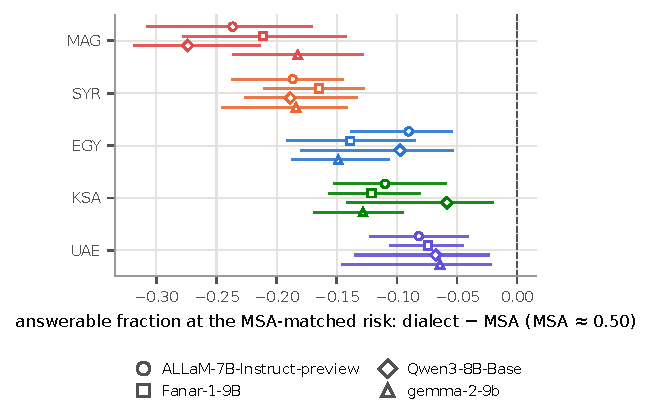
\includegraphics[width=\textwidth,height=0.43\textheight,keepaspectratio]{figures/figP1_matched_risk.pdf}
\caption{P1 sample differences from the actual MSA answerable fraction, with 95\% percentile intervals. MSA P1 is approximately 0.50; the risk reference is defined at 50\% answered.}\label{fig:p1}
\end{figure}

% Generated by tools/make_appendix_tables.py; do not edit data cells.
\begingroup
\setstretch{1}\small\setlength{\tabcolsep}{3pt}
\setlength{\LTleft}{0pt plus 1fill}\setlength{\LTright}{0pt plus 1fill}\setlength{\LTcapwidth}{\linewidth}
\setlength{\LTpre}{8pt}\setlength{\LTpost}{8pt}
\begin{longtable}{@{}>{\raggedright\arraybackslash}p{\dimexpr 0.1285700\linewidth-1.7142857\tabcolsep\relax}>{\raggedright\arraybackslash}p{\dimexpr 0.0857100\linewidth-1.7142857\tabcolsep\relax}>{\raggedright\arraybackslash}p{\dimexpr 0.1000000\linewidth-1.7142857\tabcolsep\relax}>{\raggedright\arraybackslash}p{\dimexpr 0.2285700\linewidth-1.7142857\tabcolsep\relax}>{\raggedright\arraybackslash}p{\dimexpr 0.2285700\linewidth-1.7142857\tabcolsep\relax}>{\raggedright\arraybackslash}p{\dimexpr 0.1142900\linewidth-1.7142857\tabcolsep\relax}>{\raggedright\arraybackslash}p{\dimexpr 0.1142900\linewidth-1.7142857\tabcolsep\relax}@{}}
\caption{P2 at nominal coverage 0.70: sample transferred-coverage difference $\Delta C$; fixed and double intervals; achieved own-quantile coverage $C_{\rm own}$; own-quantile set-size ratio to MSA. Values are proportions, except the ratio.}\label{tab:p2coverage}\\
\toprule
Model & Var. & $\Delta C$ & Fixed CI & Double CI & $C_{\rm own}$ & Size ratio \\
\midrule
\endfirsthead
\multicolumn{7}{l}{\small\itshape Table~\thetable\ (continued)}\\
\toprule
Model & Var. & $\Delta C$ & Fixed CI & Double CI & $C_{\rm own}$ & Size ratio \\
\midrule
\endhead
\midrule\endfoot
\bottomrule\endlastfoot
ALLaM & MAG & $-0.075$ & $[-0.098,\,-0.051]$ & $[-0.103,\,-0.047]$ & $0.657$ & $1.170$ \\*
ALLaM & SYR & $-0.063$ & $[-0.087,\,-0.039]$ & $[-0.089,\,-0.039]$ & $0.692$ & $1.204$ \\
ALLaM & EGY & $-0.037$ & $[-0.058,\,-0.015]$ & $[-0.061,\,-0.013]$ & $0.685$ & $1.107$ \\
ALLaM & KSA & $-0.047$ & $[-0.068,\,-0.027]$ & $[-0.066,\,-0.023]$ & $0.677$ & $1.116$ \\
ALLaM & UAE & $-0.043$ & $[-0.063,\,-0.023]$ & $[-0.066,\,-0.025]$ & $0.666$ & $1.076$ \\
Fanar & MAG & $-0.104$ & $[-0.127,\,-0.081]$ & $[-0.130,\,-0.071]$ & $0.692$ & $1.253$ \\
Fanar & SYR & $-0.080$ & $[-0.101,\,-0.059]$ & $[-0.107,\,-0.057]$ & $0.676$ & $1.180$ \\
Fanar & EGY & $-0.034$ & $[-0.054,\,-0.015]$ & $[-0.055,\,-0.013]$ & $0.697$ & $1.132$ \\
Fanar & KSA & $-0.054$ & $[-0.075,\,-0.035]$ & $[-0.073,\,-0.032]$ & $0.706$ & $1.163$ \\
Fanar & UAE & $-0.032$ & $[-0.051,\,-0.014]$ & $[-0.052,\,-0.011]$ & $0.701$ & $1.124$ \\
Qwen3 & MAG & $-0.130$ & $[-0.155,\,-0.106]$ & $[-0.162,\,-0.104]$ & $0.686$ & $1.321$ \\
Qwen3 & SYR & $-0.064$ & $[-0.088,\,-0.042]$ & $[-0.097,\,-0.037]$ & $0.715$ & $1.222$ \\
Qwen3 & EGY & $-0.037$ & $[-0.058,\,-0.017]$ & $[-0.061,\,-0.018]$ & $0.721$ & $1.183$ \\
Qwen3 & KSA & $-0.030$ & $[-0.049,\,-0.011]$ & $[-0.051,\,-0.008]$ & $0.723$ & $1.171$ \\
Qwen3 & UAE & $-0.032$ & $[-0.051,\,-0.014]$ & $[-0.052,\,-0.012]$ & $0.699$ & $1.120$ \\
Gemma & MAG & $-0.081$ & $[-0.105,\,-0.058]$ & $[-0.104,\,-0.050]$ & $0.692$ & $1.211$ \\
Gemma & SYR & $-0.087$ & $[-0.110,\,-0.065]$ & $[-0.111,\,-0.058]$ & $0.702$ & $1.233$ \\
Gemma & EGY & $-0.046$ & $[-0.065,\,-0.026]$ & $[-0.067,\,-0.023]$ & $0.701$ & $1.108$ \\
Gemma & KSA & $-0.035$ & $[-0.055,\,-0.015]$ & $[-0.060,\,-0.019]$ & $0.699$ & $1.096$ \\*
Gemma & UAE & $-0.030$ & $[-0.049,\,-0.010]$ & $[-0.052,\,-0.011]$ & $0.707$ & $1.105$ \\
\end{longtable}
\endgroup


\begin{figure}[H]\centering
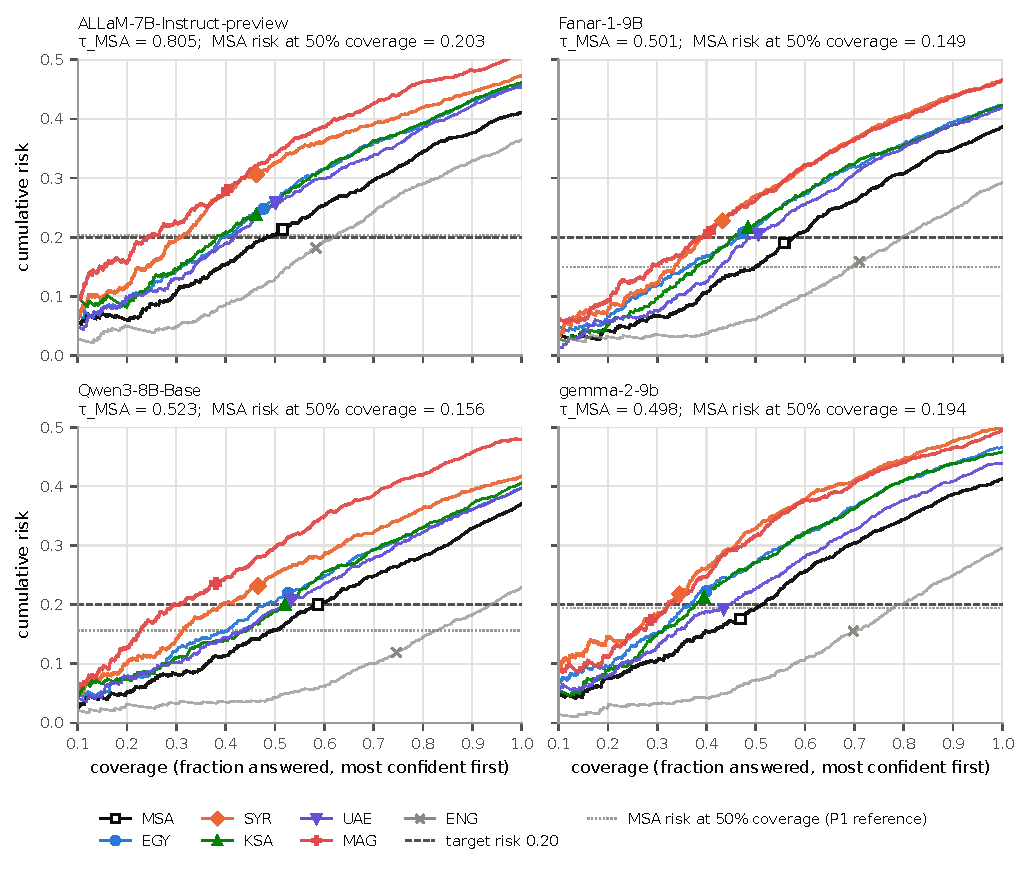
\includegraphics[width=\textwidth,height=0.43\textheight,keepaspectratio]{figures/figA_risk_coverage.pdf}
\caption{Risk--coverage curves on the 1,420 test keys. Markers indicate S4 operating points; the dotted horizontal line is the risk at MSA 50\% coverage used as the P1 reference.}\label{fig:curves}
\end{figure}

% Generated by tools/make_appendix_tables.py; do not edit data cells.
\begingroup
\setstretch{1}\small\setlength{\tabcolsep}{3pt}
\setlength{\LTleft}{0pt plus 1fill}\setlength{\LTright}{0pt plus 1fill}\setlength{\LTcapwidth}{\linewidth}
\setlength{\LTpre}{8pt}\setlength{\LTpost}{8pt}
\begin{longtable}{@{}>{\raggedright\arraybackslash}p{\dimexpr 0.1487615\linewidth-1.6666667\tabcolsep\relax}>{\raggedright\arraybackslash}p{\dimexpr 0.1074411\linewidth-1.6666667\tabcolsep\relax}>{\raggedright\arraybackslash}p{\dimexpr 0.1322313\linewidth-1.6666667\tabcolsep\relax}>{\raggedright\arraybackslash}p{\dimexpr 0.1157012\linewidth-1.6666667\tabcolsep\relax}>{\raggedright\arraybackslash}p{\dimexpr 0.2479325\linewidth-1.6666667\tabcolsep\relax}>{\raggedright\arraybackslash}p{\dimexpr 0.2479325\linewidth-1.6666667\tabcolsep\relax}@{}}
\caption{P2 mean set size and size-ratio uncertainty at nominal coverage 0.70. Ratios compare each variety with MSA using its own quantile; they do not equalise achieved coverage.}\label{tab:p2size}\\
\toprule
Model & Var. & Own size & Ratio & Fixed CI & Double CI \\
\midrule
\endfirsthead
\multicolumn{6}{l}{\small\itshape Table~\thetable\ (continued)}\\
\toprule
Model & Var. & Own size & Ratio & Fixed CI & Double CI \\
\midrule
\endhead
\midrule\endfoot
\bottomrule\endlastfoot
ALLaM & MAG & $1.532$ & $1.170$ & $[1.139,\,1.199]$ & $[1.100,\,1.294]$ \\*
ALLaM & SYR & $1.577$ & $1.204$ & $[1.173,\,1.235]$ & $[1.110,\,1.303]$ \\
ALLaM & EGY & $1.450$ & $1.107$ & $[1.082,\,1.133]$ & $[1.045,\,1.197]$ \\
ALLaM & KSA & $1.462$ & $1.116$ & $[1.093,\,1.141]$ & $[1.033,\,1.242]$ \\
ALLaM & UAE & $1.410$ & $1.076$ & $[1.052,\,1.102]$ & $[1.002,\,1.173]$ \\
Fanar & MAG & $1.542$ & $1.253$ & $[1.224,\,1.284]$ & $[1.158,\,1.385]$ \\
Fanar & SYR & $1.452$ & $1.180$ & $[1.152,\,1.207]$ & $[1.101,\,1.307]$ \\
Fanar & EGY & $1.394$ & $1.132$ & $[1.107,\,1.158]$ & $[1.058,\,1.220]$ \\
Fanar & KSA & $1.432$ & $1.163$ & $[1.137,\,1.191]$ & $[1.102,\,1.264]$ \\
Fanar & UAE & $1.383$ & $1.124$ & $[1.099,\,1.151]$ & $[1.064,\,1.214]$ \\
Qwen3 & MAG & $1.564$ & $1.321$ & $[1.289,\,1.356]$ & $[1.227,\,1.456]$ \\
Qwen3 & SYR & $1.446$ & $1.222$ & $[1.192,\,1.253]$ & $[1.135,\,1.339]$ \\
Qwen3 & EGY & $1.400$ & $1.183$ & $[1.153,\,1.213]$ & $[1.098,\,1.258]$ \\
Qwen3 & KSA & $1.387$ & $1.171$ & $[1.145,\,1.200]$ & $[1.090,\,1.241]$ \\
Qwen3 & UAE & $1.325$ & $1.120$ & $[1.094,\,1.146]$ & $[1.044,\,1.202]$ \\
Gemma & MAG & $1.720$ & $1.211$ & $[1.184,\,1.238]$ & $[1.135,\,1.322]$ \\
Gemma & SYR & $1.753$ & $1.233$ & $[1.204,\,1.262]$ & $[1.132,\,1.337]$ \\
Gemma & EGY & $1.575$ & $1.108$ & $[1.084,\,1.134]$ & $[1.043,\,1.188]$ \\
Gemma & KSA & $1.557$ & $1.096$ & $[1.071,\,1.118]$ & $[1.043,\,1.196]$ \\*
Gemma & UAE & $1.570$ & $1.105$ & $[1.080,\,1.130]$ & $[1.027,\,1.197]$ \\
\end{longtable}
\endgroup


% Generated by tools/make_appendix_tables.py; do not edit data cells.
\begingroup
\setstretch{1}\small\setlength{\tabcolsep}{3pt}
\setlength{\LTleft}{0pt plus 1fill}\setlength{\LTright}{0pt plus 1fill}\setlength{\LTcapwidth}{\linewidth}
\setlength{\LTpre}{8pt}\setlength{\LTpost}{8pt}
\begin{longtable}{@{}>{\raggedright\arraybackslash}p{\dimexpr 0.2920400\linewidth-1.6000000\tabcolsep\relax}>{\raggedright\arraybackslash}p{\dimexpr 0.1769900\linewidth-1.6000000\tabcolsep\relax}>{\raggedright\arraybackslash}p{\dimexpr 0.1769900\linewidth-1.6000000\tabcolsep\relax}>{\raggedright\arraybackslash}p{\dimexpr 0.1769900\linewidth-1.6000000\tabcolsep\relax}>{\raggedright\arraybackslash}p{\dimexpr 0.1769900\linewidth-1.6000000\tabcolsep\relax}@{}}
\caption{S2 on Moroccan at nominal coverage 0.70: achieved coverage / mean set size. All policies use the same underlying keys; pooled and group policies access more total variety rows than MSA-only. Router accuracy is 0.638.}\label{tab:s2full}\\
\toprule
Policy & ALLaM & Fanar & Qwen3 & Gemma \\
\midrule
\endfirsthead
\multicolumn{5}{l}{\small\itshape Table~\thetable\ (continued)}\\
\toprule
Policy & ALLaM & Fanar & Qwen3 & Gemma \\
\midrule
\endhead
\midrule\endfoot
\bottomrule\endlastfoot
MSA-only & $0.606\,/\,1.356$ & $0.589\,/\,1.170$ & $0.570\,/\,1.142$ & $0.624\,/\,1.437$ \\*
Pooled & $0.638\,/\,1.464$ & $0.642\,/\,1.351$ & $0.616\,/\,1.318$ & $0.655\,/\,1.558$ \\
Predicted label & $0.632\,/\,1.449$ & $0.659\,/\,1.432$ & $0.663\,/\,1.484$ & $0.684\,/\,1.670$ \\
True label & $0.657\,/\,1.532$ & $0.692\,/\,1.542$ & $0.686\,/\,1.564$ & $0.692\,/\,1.720$ \\
Plausible-set union & $0.706\,/\,1.727$ & $0.682\,/\,1.517$ & $0.686\,/\,1.564$ & $0.723\,/\,1.845$ \\*
Recovered coverage gain & $51.4\%$ & $68.3\%$ & $80.6\%$ & $87.6\%$ \\
\end{longtable}
\endgroup


% Generated by tools/make_appendix_tables.py; do not edit data cells.
\begingroup
\setstretch{1}\small\setlength{\tabcolsep}{3pt}
\setlength{\LTleft}{0pt plus 1fill}\setlength{\LTright}{0pt plus 1fill}\setlength{\LTcapwidth}{\linewidth}
\setlength{\LTpre}{8pt}\setlength{\LTpost}{8pt}
\begin{longtable}{@{}>{\raggedright\arraybackslash}p{\dimexpr 0.2000000\linewidth-1.6000000\tabcolsep\relax}>{\raggedright\arraybackslash}p{\dimexpr 0.2000000\linewidth-1.6000000\tabcolsep\relax}>{\raggedright\arraybackslash}p{\dimexpr 0.2000000\linewidth-1.6000000\tabcolsep\relax}>{\raggedright\arraybackslash}p{\dimexpr 0.2000000\linewidth-1.6000000\tabcolsep\relax}>{\raggedright\arraybackslash}p{\dimexpr 0.2000000\linewidth-1.6000000\tabcolsep\relax}@{}}
\caption{Accuracy / AUROC of $p_{\max}$ on the confirmatory test. AUROC differences and intervals are in Table~\ref{tab:3}.}\label{tab:accuracyfull}\\
\toprule
Var. & ALLaM & Fanar & Qwen3 & Gemma \\
\midrule
\endfirsthead
\multicolumn{5}{l}{\small\itshape Table~\thetable\ (continued)}\\
\toprule
Var. & ALLaM & Fanar & Qwen3 & Gemma \\
\midrule
\endhead
\midrule\endfoot
\bottomrule\endlastfoot
MSA & $0.589\,/\,0.775$ & $0.613\,/\,0.803$ & $0.630\,/\,0.796$ & $0.587\,/\,0.774$ \\*
MAG & $0.490\,/\,0.730$ & $0.535\,/\,0.764$ & $0.520\,/\,0.738$ & $0.505\,/\,0.745$ \\
SYR & $0.527\,/\,0.719$ & $0.534\,/\,0.766$ & $0.583\,/\,0.732$ & $0.499\,/\,0.738$ \\
EGY & $0.547\,/\,0.751$ & $0.577\,/\,0.766$ & $0.602\,/\,0.765$ & $0.534\,/\,0.755$ \\
KSA & $0.539\,/\,0.762$ & $0.577\,/\,0.770$ & $0.594\,/\,0.781$ & $0.542\,/\,0.747$ \\
UAE & $0.544\,/\,0.776$ & $0.580\,/\,0.790$ & $0.602\,/\,0.782$ & $0.561\,/\,0.769$ \\*
ENG & $0.635\,/\,0.806$ & $0.707\,/\,0.841$ & $0.771\,/\,0.835$ & $0.705\,/\,0.839$ \\
\end{longtable}
\endgroup


% Generated by tools/make_appendix_tables.py; do not edit data cells.
\begingroup
\setstretch{1}\small\setlength{\tabcolsep}{3pt}
\setlength{\LTleft}{0pt plus 1fill}\setlength{\LTright}{0pt plus 1fill}\setlength{\LTcapwidth}{\linewidth}
\setlength{\LTpre}{8pt}\setlength{\LTpost}{8pt}
\begin{longtable}{@{}>{\raggedright\arraybackslash}p{\dimexpr 0.1417314\linewidth-1.6666667\tabcolsep\relax}>{\raggedright\arraybackslash}p{\dimexpr 0.0944909\linewidth-1.6666667\tabcolsep\relax}>{\raggedright\arraybackslash}p{\dimexpr 0.1181112\linewidth-1.6666667\tabcolsep\relax}>{\raggedright\arraybackslash}p{\dimexpr 0.1259813\linewidth-1.6666667\tabcolsep\relax}>{\raggedright\arraybackslash}p{\dimexpr 0.2598426\linewidth-1.6666667\tabcolsep\relax}>{\raggedright\arraybackslash}p{\dimexpr 0.2598426\linewidth-1.6666667\tabcolsep\relax}@{}}
\caption{S4 answered fraction under the transferred MSA threshold at target 0.20. $A_v$ is the dialect fraction and $\Delta A=A_v-A_{\rm MSA}$.}\label{tab:s4answers}\\
\toprule
Model & Var. & $A_v$ & $\Delta A$ & Fixed CI & Double CI \\
\midrule
\endfirsthead
\multicolumn{6}{l}{\small\itshape Table~\thetable\ (continued)}\\
\toprule
Model & Var. & $A_v$ & $\Delta A$ & Fixed CI & Double CI \\
\midrule
\endhead
\midrule\endfoot
\bottomrule\endlastfoot
ALLaM & MAG & $0.403$ & $-0.113$ & $[-0.140,\,-0.087]$ & $[-0.142,\,-0.075]$ \\*
ALLaM & SYR & $0.463$ & $-0.053$ & $[-0.080,\,-0.026]$ & $[-0.088,\,-0.011]$ \\
ALLaM & EGY & $0.477$ & $-0.039$ & $[-0.063,\,-0.015]$ & $[-0.061,\,-0.004]$ \\
ALLaM & KSA & $0.462$ & $-0.054$ & $[-0.076,\,-0.030]$ & $[-0.072,\,-0.021]$ \\
ALLaM & UAE & $0.501$ & $-0.014$ & $[-0.037,\,0.009]$ & $[-0.044,\,0.014]$ \\
Fanar & MAG & $0.406$ & $-0.152$ & $[-0.177,\,-0.130]$ & $[-0.175,\,-0.120]$ \\
Fanar & SYR & $0.432$ & $-0.125$ & $[-0.150,\,-0.101]$ & $[-0.144,\,-0.092]$ \\
Fanar & EGY & $0.475$ & $-0.083$ & $[-0.106,\,-0.061]$ & $[-0.101,\,-0.056]$ \\
Fanar & KSA & $0.485$ & $-0.073$ & $[-0.096,\,-0.051]$ & $[-0.092,\,-0.050]$ \\
Fanar & UAE & $0.506$ & $-0.052$ & $[-0.073,\,-0.031]$ & $[-0.069,\,-0.024]$ \\
Qwen3 & MAG & $0.380$ & $-0.208$ & $[-0.235,\,-0.182]$ & $[-0.232,\,-0.173]$ \\
Qwen3 & SYR & $0.465$ & $-0.122$ & $[-0.147,\,-0.096]$ & $[-0.146,\,-0.094]$ \\
Qwen3 & EGY & $0.527$ & $-0.061$ & $[-0.084,\,-0.037]$ & $[-0.086,\,-0.032]$ \\
Qwen3 & KSA & $0.520$ & $-0.067$ & $[-0.089,\,-0.044]$ & $[-0.089,\,-0.039]$ \\
Qwen3 & UAE & $0.532$ & $-0.055$ & $[-0.077,\,-0.032]$ & $[-0.078,\,-0.030]$ \\
Gemma & MAG & $0.287$ & $-0.182$ & $[-0.205,\,-0.158]$ & $[-0.202,\,-0.156]$ \\
Gemma & SYR & $0.346$ & $-0.123$ & $[-0.146,\,-0.099]$ & $[-0.149,\,-0.099]$ \\
Gemma & EGY & $0.399$ & $-0.070$ & $[-0.091,\,-0.048]$ & $[-0.095,\,-0.046]$ \\
Gemma & KSA & $0.395$ & $-0.074$ & $[-0.095,\,-0.053]$ & $[-0.106,\,-0.049]$ \\*
Gemma & UAE & $0.435$ & $-0.034$ & $[-0.055,\,-0.012]$ & $[-0.060,\,-0.010]$ \\
\end{longtable}
\endgroup


% Generated by tools/make_appendix_tables.py; do not edit data cells.
\begingroup
\setstretch{1}\small\setlength{\tabcolsep}{3pt}
\setlength{\LTleft}{0pt plus 1fill}\setlength{\LTright}{0pt plus 1fill}\setlength{\LTcapwidth}{\linewidth}
\setlength{\LTpre}{8pt}\setlength{\LTpost}{8pt}
\begin{longtable}{@{}>{\raggedright\arraybackslash}p{\dimexpr 0.1417314\linewidth-1.6666667\tabcolsep\relax}>{\raggedright\arraybackslash}p{\dimexpr 0.0944909\linewidth-1.6666667\tabcolsep\relax}>{\raggedright\arraybackslash}p{\dimexpr 0.1181112\linewidth-1.6666667\tabcolsep\relax}>{\raggedright\arraybackslash}p{\dimexpr 0.1259813\linewidth-1.6666667\tabcolsep\relax}>{\raggedright\arraybackslash}p{\dimexpr 0.2598426\linewidth-1.6666667\tabcolsep\relax}>{\raggedright\arraybackslash}p{\dimexpr 0.2598426\linewidth-1.6666667\tabcolsep\relax}@{}}
\caption{S4 risk and paired risk difference from MSA. Intervals concern $\Delta R$, not exceedance of the 0.20 target. Absolute-risk intervals and both exceedance indicators are in \texttt{S101\_risk\_diff.csv}.}\label{tab:s4risk}\\
\toprule
Model & Var. & $R_v$ & $\Delta R$ & Fixed CI & Double CI \\
\midrule
\endfirsthead
\multicolumn{6}{l}{\small\itshape Table~\thetable\ (continued)}\\
\toprule
Model & Var. & $R_v$ & $\Delta R$ & Fixed CI & Double CI \\
\midrule
\endhead
\midrule\endfoot
\bottomrule\endlastfoot
ALLaM & MAG & $0.280$ & $0.067$ & $[0.031,\,0.101]$ & $[0.031,\,0.114]$ \\*
ALLaM & SYR & $0.306$ & $0.093$ & $[0.059,\,0.126]$ & $[0.053,\,0.134]$ \\
ALLaM & EGY & $0.248$ & $0.035$ & $[0.006,\,0.065]$ & $[-0.001,\,0.079]$ \\
ALLaM & KSA & $0.238$ & $0.025$ & $[-0.002,\,0.051]$ & $[0.003,\,0.061]$ \\
ALLaM & UAE & $0.258$ & $0.045$ & $[0.017,\,0.072]$ & $[0.005,\,0.073]$ \\
Fanar & MAG & $0.208$ & $0.018$ & $[-0.014,\,0.050]$ & $[-0.009,\,0.057]$ \\
Fanar & SYR & $0.228$ & $0.037$ & $[0.008,\,0.070]$ & $[0.009,\,0.079]$ \\
Fanar & EGY & $0.208$ & $0.017$ & $[-0.010,\,0.044]$ & $[-0.005,\,0.050]$ \\
Fanar & KSA & $0.217$ & $0.026$ & $[-0.001,\,0.052]$ & $[0.000,\,0.054]$ \\
Fanar & UAE & $0.205$ & $0.014$ & $[-0.010,\,0.038]$ & $[-0.009,\,0.047]$ \\
Qwen3 & MAG & $0.236$ & $0.035$ & $[0.003,\,0.070]$ & $[0.002,\,0.072]$ \\
Qwen3 & SYR & $0.231$ & $0.031$ & $[0.003,\,0.061]$ & $[0.003,\,0.067]$ \\
Qwen3 & EGY & $0.219$ & $0.019$ & $[-0.005,\,0.044]$ & $[-0.005,\,0.047]$ \\
Qwen3 & KSA & $0.200$ & $0.000$ & $[-0.024,\,0.025]$ & $[-0.023,\,0.034]$ \\
Qwen3 & UAE & $0.208$ & $0.007$ & $[-0.017,\,0.033]$ & $[-0.020,\,0.030]$ \\
Gemma & MAG & $0.174$ & $-0.002$ & $[-0.036,\,0.035]$ & $[-0.039,\,0.035]$ \\
Gemma & SYR & $0.218$ & $0.042$ & $[0.010,\,0.077]$ & $[0.000,\,0.084]$ \\
Gemma & EGY & $0.222$ & $0.047$ & $[0.017,\,0.076]$ & $[0.009,\,0.078]$ \\
Gemma & KSA & $0.212$ & $0.036$ & $[0.011,\,0.061]$ & $[-0.006,\,0.066]$ \\*
Gemma & UAE & $0.193$ & $0.017$ & $[-0.009,\,0.044]$ & $[-0.009,\,0.048]$ \\
\end{longtable}
\endgroup


% Generated by tools/make_appendix_tables.py; do not edit data cells.
\begingroup
\setstretch{1}\small\setlength{\tabcolsep}{3pt}
\setlength{\LTleft}{0pt plus 1fill}\setlength{\LTright}{0pt plus 1fill}\setlength{\LTcapwidth}{\linewidth}
\setlength{\LTpre}{8pt}\setlength{\LTpost}{8pt}
\begin{longtable}{@{}>{\raggedright\arraybackslash}p{\dimexpr 0.1393400\linewidth-1.7142857\tabcolsep\relax}>{\raggedright\arraybackslash}p{\dimexpr 0.0901600\linewidth-1.7142857\tabcolsep\relax}>{\raggedright\arraybackslash}p{\dimexpr 0.1311500\linewidth-1.7142857\tabcolsep\relax}>{\raggedright\arraybackslash}p{\dimexpr 0.1311500\linewidth-1.7142857\tabcolsep\relax}>{\raggedright\arraybackslash}p{\dimexpr 0.1311500\linewidth-1.7142857\tabcolsep\relax}>{\raggedright\arraybackslash}p{\dimexpr 0.1311500\linewidth-1.7142857\tabcolsep\relax}>{\raggedright\arraybackslash}p{\dimexpr 0.2459000\linewidth-1.7142857\tabcolsep\relax}@{}}
\caption{D4 at target 0.20: answered fractions and risks before (MSA threshold) and after (own threshold) adaptation. The final interval is fixed-calibration uncertainty for adapted risk.}\label{tab:d4points}\\
\toprule
Model & Var. & $A_{\rm before}$ & $A_{\rm after}$ & $R_{\rm before}$ & $R_{\rm after}$ & After-risk CI \\
\midrule
\endfirsthead
\multicolumn{7}{l}{\small\itshape Table~\thetable\ (continued)}\\
\toprule
Model & Var. & $A_{\rm before}$ & $A_{\rm after}$ & $R_{\rm before}$ & $R_{\rm after}$ & After-risk CI \\
\midrule
\endhead
\midrule\endfoot
\bottomrule\endlastfoot
ALLaM & MAG & $0.403$ & $0.235$ & $0.280$ & $0.195$ & $[0.154,\,0.238]$ \\*
ALLaM & SYR & $0.463$ & $0.354$ & $0.306$ & $0.237$ & $[0.199,\,0.275]$ \\
ALLaM & EGY & $0.477$ & $0.396$ & $0.248$ & $0.199$ & $[0.168,\,0.235]$ \\
ALLaM & KSA & $0.462$ & $0.369$ & $0.238$ & $0.187$ & $[0.154,\,0.222]$ \\
ALLaM & UAE & $0.501$ & $0.376$ & $0.258$ & $0.176$ & $[0.143,\,0.210]$ \\
Fanar & MAG & $0.406$ & $0.366$ & $0.208$ & $0.188$ & $[0.155,\,0.222]$ \\
Fanar & SYR & $0.432$ & $0.360$ & $0.228$ & $0.174$ & $[0.143,\,0.207]$ \\
Fanar & EGY & $0.475$ & $0.519$ & $0.208$ & $0.231$ & $[0.200,\,0.261]$ \\
Fanar & KSA & $0.485$ & $0.457$ & $0.217$ & $0.202$ & $[0.172,\,0.233]$ \\
Fanar & UAE & $0.506$ & $0.499$ & $0.205$ & $0.202$ & $[0.173,\,0.232]$ \\
Qwen3 & MAG & $0.380$ & $0.247$ & $0.236$ & $0.171$ & $[0.133,\,0.210]$ \\
Qwen3 & SYR & $0.465$ & $0.391$ & $0.231$ & $0.198$ & $[0.167,\,0.229]$ \\
Qwen3 & EGY & $0.527$ & $0.417$ & $0.219$ & $0.166$ & $[0.136,\,0.196]$ \\
Qwen3 & KSA & $0.520$ & $0.512$ & $0.200$ & $0.194$ & $[0.166,\,0.222]$ \\
Qwen3 & UAE & $0.532$ & $0.501$ & $0.208$ & $0.191$ & $[0.163,\,0.219]$ \\
Gemma & MAG & $0.287$ & $0.279$ & $0.174$ & $0.164$ & $[0.129,\,0.202]$ \\
Gemma & SYR & $0.346$ & $0.267$ & $0.218$ & $0.164$ & $[0.128,\,0.202]$ \\
Gemma & EGY & $0.399$ & $0.390$ & $0.222$ & $0.222$ & $[0.189,\,0.258]$ \\
Gemma & KSA & $0.395$ & $0.397$ & $0.212$ & $0.215$ & $[0.181,\,0.251]$ \\*
Gemma & UAE & $0.435$ & $0.459$ & $0.193$ & $0.209$ & $[0.178,\,0.241]$ \\
\end{longtable}
\endgroup


% Generated by tools/make_appendix_tables.py; do not edit data cells.
\begingroup
\setstretch{1}\small\setlength{\tabcolsep}{3pt}
\setlength{\LTleft}{0pt plus 1fill}\setlength{\LTright}{0pt plus 1fill}\setlength{\LTcapwidth}{\linewidth}
\setlength{\LTpre}{8pt}\setlength{\LTpost}{8pt}
\begin{longtable}{@{}>{\raggedright\arraybackslash}p{\dimexpr 0.1176488\linewidth-1.6666667\tabcolsep\relax}>{\raggedright\arraybackslash}p{\dimexpr 0.0808792\linewidth-1.6666667\tabcolsep\relax}>{\raggedright\arraybackslash}p{\dimexpr 0.2720573\linewidth-1.6666667\tabcolsep\relax}>{\raggedright\arraybackslash}p{\dimexpr 0.1029390\linewidth-1.6666667\tabcolsep\relax}>{\raggedright\arraybackslash}p{\dimexpr 0.2132379\linewidth-1.6666667\tabcolsep\relax}>{\raggedright\arraybackslash}p{\dimexpr 0.2132379\linewidth-1.6666667\tabcolsep\relax}@{}}
\caption{D4 change in answered fraction after adaptation and residual difference from MSA at the same nominal target. The change column includes its fixed interval; residual intervals are shown both ways. The full double-resampled adapted-risk intervals are in \texttt{S91\_calibration\_sensitivity.csv}.}\label{tab:d4gaps}\\
\toprule
Model & Var. & Change [fixed CI] & Residual & Fixed CI & Double CI \\
\midrule
\endfirsthead
\multicolumn{6}{l}{\small\itshape Table~\thetable\ (continued)}\\
\toprule
Model & Var. & Change [fixed CI] & Residual & Fixed CI & Double CI \\
\midrule
\endhead
\midrule\endfoot
\bottomrule\endlastfoot
ALLaM & MAG & $-0.168\;[-0.187,\,-0.149]$ & $-0.280$ & $[-0.306,\,-0.254]$ & $[-0.358,\,-0.175]$ \\*
ALLaM & SYR & $-0.109\;[-0.125,\,-0.094]$ & $-0.162$ & $[-0.189,\,-0.136]$ & $[-0.284,\,-0.082]$ \\
ALLaM & EGY & $-0.081\;[-0.096,\,-0.067]$ & $-0.120$ & $[-0.144,\,-0.096]$ & $[-0.218,\,-0.029]$ \\
ALLaM & KSA & $-0.093\;[-0.108,\,-0.078]$ & $-0.146$ & $[-0.170,\,-0.123]$ & $[-0.231,\,-0.051]$ \\
ALLaM & UAE & $-0.125\;[-0.144,\,-0.108]$ & $-0.139$ & $[-0.163,\,-0.116]$ & $[-0.227,\,-0.051]$ \\
Fanar & MAG & $-0.039\;[-0.050,\,-0.030]$ & $-0.192$ & $[-0.217,\,-0.167]$ & $[-0.290,\,-0.108]$ \\
Fanar & SYR & $-0.073\;[-0.086,\,-0.060]$ & $-0.198$ & $[-0.222,\,-0.174]$ & $[-0.269,\,-0.088]$ \\
Fanar & EGY & $0.044\;[0.034,\,0.056]$ & $-0.039$ & $[-0.061,\,-0.017]$ & $[-0.118,\,0.044]$ \\
Fanar & KSA & $-0.027\;[-0.037,\,-0.020]$ & $-0.101$ & $[-0.123,\,-0.080]$ & $[-0.175,\,-0.022]$ \\
Fanar & UAE & $-0.007\;[-0.012,\,-0.003]$ & $-0.059$ & $[-0.080,\,-0.039]$ & $[-0.140,\,0.013]$ \\
Qwen3 & MAG & $-0.132\;[-0.150,\,-0.115]$ & $-0.340$ & $[-0.368,\,-0.314]$ & $[-0.424,\,-0.177]$ \\
Qwen3 & SYR & $-0.075\;[-0.089,\,-0.061]$ & $-0.196$ & $[-0.223,\,-0.169]$ & $[-0.275,\,-0.076]$ \\
Qwen3 & EGY & $-0.110\;[-0.127,\,-0.094]$ & $-0.170$ & $[-0.194,\,-0.146]$ & $[-0.254,\,-0.066]$ \\
Qwen3 & KSA & $-0.008\;[-0.013,\,-0.004]$ & $-0.075$ & $[-0.098,\,-0.054]$ & $[-0.154,\,0.012]$ \\
Qwen3 & UAE & $-0.032\;[-0.042,\,-0.023]$ & $-0.087$ & $[-0.109,\,-0.064]$ & $[-0.168,\,0.024]$ \\
Gemma & MAG & $-0.008\;[-0.013,\,-0.004]$ & $-0.190$ & $[-0.214,\,-0.168]$ & $[-0.258,\,-0.154]$ \\
Gemma & SYR & $-0.079\;[-0.093,\,-0.065]$ & $-0.202$ & $[-0.227,\,-0.180]$ & $[-0.279,\,-0.111]$ \\
Gemma & EGY & $-0.009\;[-0.014,\,-0.004]$ & $-0.079$ & $[-0.100,\,-0.058]$ & $[-0.139,\,0.006]$ \\
Gemma & KSA & $0.002\;[0.000,\,0.005]$ & $-0.072$ & $[-0.092,\,-0.051]$ & $[-0.143,\,-0.020]$ \\*
Gemma & UAE & $0.024\;[0.016,\,0.032]$ & $-0.010$ & $[-0.031,\,0.011]$ & $[-0.092,\,0.049]$ \\
\end{longtable}
\endgroup


% Generated by tools/make_appendix_tables.py; do not edit data cells.
\begingroup
\setstretch{1}\small\setlength{\tabcolsep}{3pt}
\setlength{\LTleft}{0pt plus 1fill}\setlength{\LTright}{0pt plus 1fill}\setlength{\LTcapwidth}{\linewidth}
\setlength{\LTpre}{8pt}\setlength{\LTpost}{8pt}
\begin{longtable}{@{}>{\raggedright\arraybackslash}p{\dimexpr 0.1118911\linewidth-1.6666667\tabcolsep\relax}>{\raggedright\arraybackslash}p{\dimexpr 0.0769208\linewidth-1.6666667\tabcolsep\relax}>{\raggedright\arraybackslash}p{\dimexpr 0.2377624\linewidth-1.6666667\tabcolsep\relax}>{\raggedright\arraybackslash}p{\dimexpr 0.2377624\linewidth-1.6666667\tabcolsep\relax}>{\raggedright\arraybackslash}p{\dimexpr 0.2377624\linewidth-1.6666667\tabcolsep\relax}>{\raggedright\arraybackslash}p{\dimexpr 0.0979010\linewidth-1.6666667\tabcolsep\relax}@{}}
\caption{AraDiCE: 1,400 test keys; paired differences from MSA in accuracy, P1 and coverage under the MSA quantile ($\alpha=0.30$), with fixed-calibration intervals. Own-quantile size ratios are point estimates.}\label{tab:aradice}\\
\toprule
Model & Var. & $\Delta$ accuracy & $\Delta$ P1 & $\Delta$ coverage & Size ratio \\
\midrule
\endfirsthead
\multicolumn{6}{l}{\small\itshape Table~\thetable\ (continued)}\\
\toprule
Model & Var. & $\Delta$ accuracy & $\Delta$ P1 & $\Delta$ coverage & Size ratio \\
\midrule
\endhead
\midrule\endfoot
\bottomrule\endlastfoot
ALLaM & EGY & $-0.070$\newline$[-0.092,\,-0.048]$ & $-0.172$\newline$[-0.242,\,-0.127]$ & $-0.067$\newline$[-0.089,\,-0.045]$ & $1.276$ \\*
ALLaM & LEV & $-0.045$\newline$[-0.066,\,-0.026]$ & $-0.137$\newline$[-0.172,\,-0.090]$ & $-0.051$\newline$[-0.071,\,-0.032]$ & $1.158$ \\
Fanar & EGY & $-0.045$\newline$[-0.066,\,-0.024]$ & $-0.109$\newline$[-0.163,\,-0.065]$ & $-0.037$\newline$[-0.058,\,-0.016]$ & $1.177$ \\
Fanar & LEV & $-0.037$\newline$[-0.056,\,-0.017]$ & $-0.060$\newline$[-0.101,\,-0.037]$ & $-0.052$\newline$[-0.071,\,-0.033]$ & $1.047$ \\
Qwen3 & EGY & $-0.046$\newline$[-0.068,\,-0.023]$ & $-0.151$\newline$[-0.211,\,-0.101]$ & $-0.059$\newline$[-0.078,\,-0.038]$ & $1.214$ \\
Qwen3 & LEV & $-0.036$\newline$[-0.055,\,-0.016]$ & $-0.104$\newline$[-0.150,\,-0.059]$ & $-0.042$\newline$[-0.061,\,-0.025]$ & $1.017$ \\
Gemma & EGY & $-0.052$\newline$[-0.074,\,-0.031]$ & $-0.135$\newline$[-0.172,\,-0.094]$ & $-0.056$\newline$[-0.076,\,-0.035]$ & $1.206$ \\*
Gemma & LEV & $-0.036$\newline$[-0.056,\,-0.016]$ & $-0.092$\newline$[-0.131,\,-0.057]$ & $-0.033$\newline$[-0.052,\,-0.013]$ & $1.088$ \\
\end{longtable}
\endgroup


The supplementary result grids contain the remaining operating points: all four S4 target risks, eight P2 error levels, both S2 error levels and all seven varieties. D1/D2 contains the discrimination estimates, D4 the adaptation results, and S91 the calibration-resampling results at the principal targets. L1 and L2 contain the external-filter and embedding-stratified analyses. The file index (\nolinkurl{docs/FILE_INDEX.md}) in the supplementary source archive maps these tables to their archived CSVs.

\FloatBarrier
\section{Computational verification and numerical precision}\label{independent-computational-check}

A separate implementation computed P1, S4 and P2 from the written metric definitions and stored scores without consulting the original analysis code or reports, according to the archived comparison record. Table~\ref{tab:indep} summarises the agreement. This checks implementation of the metrics on shared inputs; it does not independently validate model scoring or equivalence of the question versions.

% Generated by tools/make_appendix_tables.py; do not edit data cells.
\begingroup
\setstretch{1}\small\setlength{\tabcolsep}{3pt}
\setlength{\LTleft}{0pt plus 1fill}\setlength{\LTright}{0pt plus 1fill}\setlength{\LTcapwidth}{\linewidth}
\setlength{\LTpre}{8pt}\setlength{\LTpost}{8pt}
\begin{longtable}{@{}>{\raggedright\arraybackslash}p{\dimexpr 0.3200000\linewidth-1.5000000\tabcolsep\relax}>{\raggedright\arraybackslash}p{\dimexpr 0.1000000\linewidth-1.5000000\tabcolsep\relax}>{\raggedright\arraybackslash}p{\dimexpr 0.3200000\linewidth-1.5000000\tabcolsep\relax}>{\raggedright\arraybackslash}p{\dimexpr 0.2600000\linewidth-1.5000000\tabcolsep\relax}@{}}
\caption{Agreement between the separate metric implementation and the original results.}\label{tab:indep}\\
\toprule
Quantity & Cells & Maximum absolute difference & Interpretation \\
\midrule
\endfirsthead
\multicolumn{4}{l}{\small\itshape Table~\thetable\ (continued)}\\
\toprule
Quantity & Cells & Maximum absolute difference & Interpretation \\
\midrule
\endhead
\midrule\endfoot
\bottomrule\endlastfoot
P1: t50 and answerable fraction, all varieties & 28 & 0.0 & identical \\*
S4: $\tau$, answered fraction, realised risk at r* = 0.15 / 0.20 / 0.25 & 84 & $\tau$ $\leq$ 1e-5; fractions $\leq$ 7.0e-4 (= one item of 1,420); risk $\leq$ 1.0e-3 & agree to one boundary item \\
S4 at r* = 0.30 & 28 & $\tau$ 3.3e-3 (Fanar); answered $\leq$ 1.06e-2 & input-precision effect, see below \\
P2 ($\alpha$ = 0.20, 0.30): $\hat q$, coverage under MSA $\hat q$, $\Delta C$, size under MSA $\hat q$ & 56 & $\leq$ 1.5e-3 & agree to 1--2 boundary items \\
P2: coverage and size under own $\hat q$, size ratio & 56 & size $\leq$ 8.5e-3; ratio $\leq$ 7.1e-3 & boundary items at the rounded log-probabilities \\
per-key S4 answered indicator (r* = 0.20), 4 $\times$ 9,940 cells & 39,760 & 1 mismatch (Fanar) & agree \\*
per-key conformal coverage indicator ($\alpha$ = 0.30) & 39,760 & 5 mismatches in total & agree \\
\end{longtable}
\endgroup


The main analysis uses stored $p_{\max}$ and $p_{\mathrm{true}}$ values rounded to five decimals, whereas the separate implementation primarily reconstructs them from letter log-probabilities rounded to four decimals. Near-tied calibration items can therefore change rank or cross a threshold. P1 and S4 use NumPy's default sort; AUGRC uses a stable sort. Acceptance includes all items tied at the chosen threshold. The archived clean-folder check reported 51 of 57 files identical or numerically equal. A further submission audit reproduced the S4, P2 and S2 result tables, P1 point estimates and D4 results at the primary 0.20 target. Some resampled intervals and secondary D4 operating points differed across environments; the supplementary audit records these differences, including a 0.020 change in one secondary-target risk estimate. These checks concern stored inputs. Full-precision scores, explicit tie handling and a pinned software environment would improve future reproducibility.

The earlier draft displayed bootstrap-mean contrasts. Following a Codex-assisted numerical check, these were corrected to observed-sample differences, such as $A_v-A_{\mathrm{MSA}}$ for P1, while retaining the original percentile bootstrap intervals. Six P1 values change at two-decimal display precision: ALLaM--EGY ($-0.10$ to $-0.09$), Fanar--MAG ($-0.20$ to $-0.21$), Fanar--SYR ($-0.17$ to $-0.16$), Qwen3--EGY ($-0.11$ to $-0.10$), Gemma--SYR ($-0.19$ to $-0.18$) and Gemma--UAE ($-0.08$ to $-0.06$). For Gemma--UAE, the sample difference is $0.437324-0.501408=-0.064085$; the mean bootstrap difference is $-0.077917$. These estimators need not coincide because the largest admissible prefix is a nonlinear statistic. S4 answered-fraction and P2 coverage contrasts are also computed from the sample quantities. The reporting history preserves the former centres; raw scores and thresholds are unchanged, as are the P1, S4 and P2 interval endpoints.

Archived source documents the prompt, candidate-letter aggregation, sorting and stored precision. The model identifiers are \nolinkurl{ALLaM-AI/ALLaM-7B-Instruct-preview}, \nolinkurl{QCRI/Fanar-1-9B}, \nolinkurl{Qwen/Qwen3-8B-Base} and \nolinkurl{google/gemma-2-9b}. Original immutable model revisions and a complete dependency lock were not recorded.

\FloatBarrier
\section{Measurement robustness}\label{robustness-tables}

The robustness subset contains 500 test keys and four cyclic option rotations. The tables distinguish changes in selected options, differences averaged across rotations, agreement between answer-extraction methods, and realised risk among accepted items. They are exploratory checks specified after the main results. Tables~\ref{tab:ordersensitivity}--\ref{tab:paired} report the rotation analyses, and Tables~\ref{tab:g1} and~\ref{tab:g2} report generation checks. Full per-rotation estimates and re-scoring margin diagnostics are supplied in the original R1--R5 and S92 CSV files.

% Generated by tools/make_appendix_tables.py; do not edit data cells.
\begingroup
\setstretch{1}\small\setlength{\tabcolsep}{3pt}
\setlength{\LTleft}{0pt plus 1fill}\setlength{\LTright}{0pt plus 1fill}\setlength{\LTcapwidth}{\linewidth}
\setlength{\LTpre}{8pt}\setlength{\LTpost}{8pt}
\begin{longtable}{@{}>{\raggedright\arraybackslash}p{\dimexpr 0.0977420\linewidth-1.6000000\tabcolsep\relax}>{\raggedright\arraybackslash}p{\dimexpr 0.2255645\linewidth-1.6000000\tabcolsep\relax}>{\raggedright\arraybackslash}p{\dimexpr 0.2255645\linewidth-1.6000000\tabcolsep\relax}>{\raggedright\arraybackslash}p{\dimexpr 0.2255645\linewidth-1.6000000\tabcolsep\relax}>{\raggedright\arraybackslash}p{\dimexpr 0.2255645\linewidth-1.6000000\tabcolsep\relax}@{}}
\caption{Order-sensitivity rate / paired difference from MSA, with the 95\% interval below. Three decimal places retain the small positive endpoint for ALLaM--EGY.}\label{tab:ordersensitivity}\\
\toprule
Var. & ALLaM & Fanar & Qwen3 & Gemma \\
\midrule
\endfirsthead
\multicolumn{5}{l}{\small\itshape Table~\thetable\ (continued)}\\
\toprule
Var. & ALLaM & Fanar & Qwen3 & Gemma \\
\midrule
\endhead
\midrule\endfoot
\bottomrule\endlastfoot
MSA & $0.430$ & $0.454$ & $0.450$ & $0.582$ \\*
MAG & $0.514$ / $0.084$\newline$[0.034,\,0.132]$ & $0.610$ / $0.156$\newline$[0.112,\,0.200]$ & $0.566$ / $0.116$\newline$[0.070,\,0.166]$ & $0.716$ / $0.134$\newline$[0.088,\,0.178]$ \\
SYR & $0.516$ / $0.086$\newline$[0.042,\,0.132]$ & $0.582$ / $0.128$\newline$[0.080,\,0.174]$ & $0.524$ / $0.074$\newline$[0.030,\,0.120]$ & $0.704$ / $0.122$\newline$[0.078,\,0.166]$ \\
EGY & $0.476$ / $0.046$\newline$[0.002,\,0.090]$ & $0.520$ / $0.066$\newline$[0.024,\,0.108]$ & $0.498$ / $0.048$\newline$[0.006,\,0.092]$ & $0.640$ / $0.058$\newline$[0.020,\,0.102]$ \\
KSA & $0.482$ / $0.052$\newline$[0.010,\,0.094]$ & $0.542$ / $0.088$\newline$[0.050,\,0.126]$ & $0.486$ / $0.036$\newline$[-0.004,\,0.078]$ & $0.662$ / $0.080$\newline$[0.038,\,0.124]$ \\
UAE & $0.456$ / $0.026$\newline$[-0.014,\,0.068]$ & $0.520$ / $0.066$\newline$[0.022,\,0.108]$ & $0.482$ / $0.032$\newline$[-0.008,\,0.076]$ & $0.618$ / $0.036$\newline$[-0.004,\,0.076]$ \\*
ENG & $0.370$ / $-0.060$\newline$[-0.106,\,-0.016]$ & $0.342$ / $-0.112$\newline$[-0.158,\,-0.068]$ & $0.264$ / $-0.186$\newline$[-0.234,\,-0.138]$ & $0.374$ / $-0.208$\newline$[-0.252,\,-0.164]$ \\
\end{longtable}
\endgroup


% Generated by tools/make_appendix_tables.py; do not edit data cells.
\begingroup
\setstretch{1}\small\setlength{\tabcolsep}{3pt}
\setlength{\LTleft}{0pt plus 1fill}\setlength{\LTright}{0pt plus 1fill}\setlength{\LTcapwidth}{\linewidth}
\setlength{\LTpre}{8pt}\setlength{\LTpost}{8pt}
\begin{longtable}{@{}>{\raggedright\arraybackslash}p{\dimexpr 0.1641767\linewidth-1.6000000\tabcolsep\relax}>{\raggedright\arraybackslash}p{\dimexpr 0.2089558\linewidth-1.6000000\tabcolsep\relax}>{\raggedright\arraybackslash}p{\dimexpr 0.2089558\linewidth-1.6000000\tabcolsep\relax}>{\raggedright\arraybackslash}p{\dimexpr 0.2089558\linewidth-1.6000000\tabcolsep\relax}>{\raggedright\arraybackslash}p{\dimexpr 0.2089558\linewidth-1.6000000\tabcolsep\relax}@{}}
\caption{Differences from MSA averaged over four rotations, with paired key-bootstrap intervals. Every difference keeps its sign under all four rotations.}\label{tab:rotationgaps}\\
\toprule
Var. / quantity & ALLaM & Fanar & Qwen3 & Gemma \\
\midrule
\endfirsthead
\multicolumn{5}{l}{\small\itshape Table~\thetable\ (continued)}\\
\toprule
Var. / quantity & ALLaM & Fanar & Qwen3 & Gemma \\
\midrule
\endhead
\midrule\endfoot
\bottomrule\endlastfoot
MAG / Accuracy & $-0.093$\newline$[-0.122,\,-0.067]$ & $-0.115$\newline$[-0.144,\,-0.088]$ & $-0.135$\newline$[-0.167,\,-0.105]$ & $-0.110$\newline$[-0.138,\,-0.083]$ \\*
MAG / P1 & $-0.206$\newline$[-0.285,\,-0.147]$ & $-0.224$\newline$[-0.280,\,-0.165]$ & $-0.253$\newline$[-0.316,\,-0.208]$ & $-0.237$\newline$[-0.291,\,-0.178]$ \\
SYR / Accuracy & $-0.073$\newline$[-0.102,\,-0.046]$ & $-0.082$\newline$[-0.113,\,-0.056]$ & $-0.074$\newline$[-0.104,\,-0.044]$ & $-0.108$\newline$[-0.135,\,-0.080]$ \\
SYR / P1 & $-0.192$\newline$[-0.259,\,-0.139]$ & $-0.204$\newline$[-0.297,\,-0.135]$ & $-0.195$\newline$[-0.318,\,-0.117]$ & $-0.248$\newline$[-0.339,\,-0.189]$ \\
EGY / Accuracy & $-0.026$\newline$[-0.051,\,-0.003]$ & $-0.052$\newline$[-0.076,\,-0.027]$ & $-0.055$\newline$[-0.080,\,-0.031]$ & $-0.066$\newline$[-0.089,\,-0.043]$ \\
EGY / P1 & $-0.130$\newline$[-0.211,\,-0.069]$ & $-0.153$\newline$[-0.221,\,-0.093]$ & $-0.142$\newline$[-0.222,\,-0.074]$ & $-0.150$\newline$[-0.212,\,-0.106]$ \\
KSA / Accuracy & $-0.053$\newline$[-0.079,\,-0.029]$ & $-0.042$\newline$[-0.064,\,-0.021]$ & $-0.046$\newline$[-0.074,\,-0.020]$ & $-0.069$\newline$[-0.094,\,-0.045]$ \\
KSA / P1 & $-0.097$\newline$[-0.174,\,-0.049]$ & $-0.123$\newline$[-0.186,\,-0.055]$ & $-0.121$\newline$[-0.201,\,-0.043]$ & $-0.153$\newline$[-0.217,\,-0.113]$ \\
UAE / Accuracy & $-0.033$\newline$[-0.058,\,-0.010]$ & $-0.048$\newline$[-0.072,\,-0.024]$ & $-0.042$\newline$[-0.068,\,-0.017]$ & $-0.054$\newline$[-0.078,\,-0.031]$ \\*
UAE / P1 & $-0.076$\newline$[-0.144,\,-0.013]$ & $-0.104$\newline$[-0.169,\,-0.053]$ & $-0.089$\newline$[-0.172,\,-0.035]$ & $-0.131$\newline$[-0.191,\,-0.063]$ \\
\end{longtable}
\endgroup


% Generated by tools/make_appendix_tables.py; do not edit data cells.
\begingroup
\setstretch{1}\small\setlength{\tabcolsep}{3pt}
\setlength{\LTleft}{0pt plus 1fill}\setlength{\LTright}{0pt plus 1fill}\setlength{\LTcapwidth}{\linewidth}
\setlength{\LTpre}{8pt}\setlength{\LTpost}{8pt}
\begin{longtable}{@{}>{\raggedright\arraybackslash}p{\dimexpr 0.1230788\linewidth-1.6666667\tabcolsep\relax}>{\raggedright\arraybackslash}p{\dimexpr 0.0923091\linewidth-1.6666667\tabcolsep\relax}>{\raggedright\arraybackslash}p{\dimexpr 0.1076889\linewidth-1.6666667\tabcolsep\relax}>{\raggedright\arraybackslash}p{\dimexpr 0.1076889\linewidth-1.6666667\tabcolsep\relax}>{\raggedright\arraybackslash}p{\dimexpr 0.2846172\linewidth-1.6666667\tabcolsep\relax}>{\raggedright\arraybackslash}p{\dimexpr 0.2846172\linewidth-1.6666667\tabcolsep\relax}@{}}
\caption{Paired rotation comparison. $D$ is cross-version answer-change indicator minus within-variety one-rotation change; $D^\prime$ uses MSA one-rotation change as the comparator.}\label{tab:paired}\\
\toprule
Model & Var. & P3 & Within & $D$ [CI] & $D^\prime$ [CI] \\
\midrule
\endfirsthead
\multicolumn{6}{l}{\small\itshape Table~\thetable\ (continued)}\\
\toprule
Model & Var. & P3 & Within & $D$ [CI] & $D^\prime$ [CI] \\
\midrule
\endhead
\midrule\endfoot
\bottomrule\endlastfoot
ALLaM & MAG & $0.324$ & $0.312$ & $0.012\;[-0.038,\,0.060]$ & $0.058\;[0.008,\,0.106]$ \\*
ALLaM & SYR & $0.314$ & $0.286$ & $0.028\;[-0.020,\,0.076]$ & $0.048\;[0.002,\,0.098]$ \\
ALLaM & EGY & $0.246$ & $0.262$ & $-0.016\;[-0.060,\,0.030]$ & $-0.020\;[-0.062,\,0.024]$ \\
ALLaM & KSA & $0.228$ & $0.304$ & $-0.076\;[-0.124,\,-0.028]$ & $-0.038\;[-0.084,\,0.008]$ \\
ALLaM & UAE & $0.234$ & $0.240$ & $-0.006\;[-0.052,\,0.040]$ & $-0.032\;[-0.078,\,0.012]$ \\
Fanar & MAG & $0.306$ & $0.392$ & $-0.086\;[-0.140,\,-0.038]$ & $0.022\;[-0.034,\,0.072]$ \\
Fanar & SYR & $0.286$ & $0.388$ & $-0.102\;[-0.158,\,-0.048]$ & $0.002\;[-0.048,\,0.054]$ \\
Fanar & EGY & $0.252$ & $0.356$ & $-0.104\;[-0.150,\,-0.056]$ & $-0.032\;[-0.084,\,0.020]$ \\
Fanar & KSA & $0.210$ & $0.352$ & $-0.142\;[-0.188,\,-0.096]$ & $-0.074\;[-0.122,\,-0.026]$ \\
Fanar & UAE & $0.256$ & $0.316$ & $-0.060\;[-0.108,\,-0.012]$ & $-0.028\;[-0.078,\,0.020]$ \\
Qwen3 & MAG & $0.290$ & $0.368$ & $-0.078\;[-0.130,\,-0.024]$ & $0.002\;[-0.054,\,0.056]$ \\
Qwen3 & SYR & $0.288$ & $0.322$ & $-0.034\;[-0.086,\,0.018]$ & $0.000\;[-0.050,\,0.052]$ \\
Qwen3 & EGY & $0.198$ & $0.306$ & $-0.108\;[-0.156,\,-0.060]$ & $-0.090\;[-0.142,\,-0.038]$ \\
Qwen3 & KSA & $0.208$ & $0.290$ & $-0.082\;[-0.132,\,-0.032]$ & $-0.080\;[-0.132,\,-0.030]$ \\
Qwen3 & UAE & $0.214$ & $0.312$ & $-0.098\;[-0.150,\,-0.048]$ & $-0.074\;[-0.124,\,-0.024]$ \\
Gemma & MAG & $0.314$ & $0.484$ & $-0.170\;[-0.224,\,-0.116]$ & $-0.066\;[-0.122,\,-0.010]$ \\
Gemma & SYR & $0.332$ & $0.458$ & $-0.126\;[-0.178,\,-0.072]$ & $-0.048\;[-0.106,\,0.012]$ \\
Gemma & EGY & $0.244$ & $0.412$ & $-0.168\;[-0.218,\,-0.120]$ & $-0.136\;[-0.188,\,-0.082]$ \\
Gemma & KSA & $0.230$ & $0.424$ & $-0.194\;[-0.246,\,-0.138]$ & $-0.150\;[-0.204,\,-0.096]$ \\*
Gemma & UAE & $0.230$ & $0.418$ & $-0.188\;[-0.240,\,-0.138]$ & $-0.150\;[-0.202,\,-0.096]$ \\
\end{longtable}
\endgroup


\begin{figure}[H]\centering
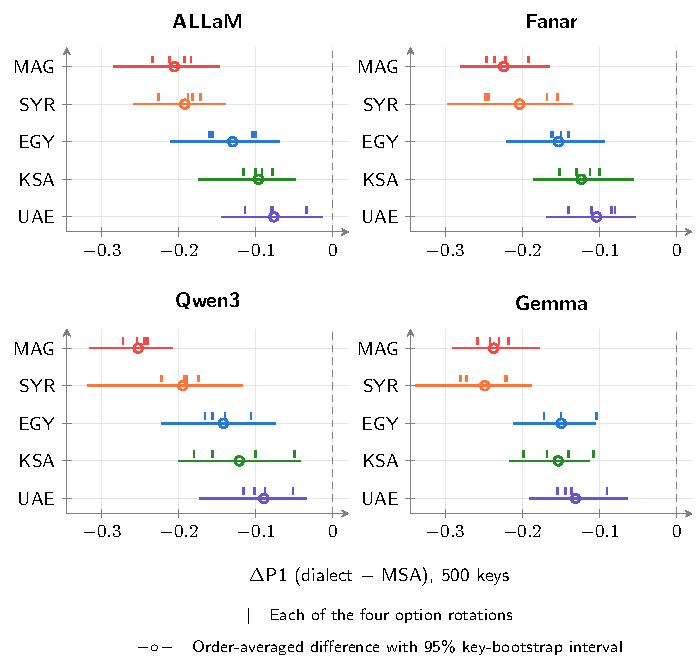
\includegraphics[width=0.94\textwidth]{figures/figB_rotations.pdf}
\caption{P1 differences for each of four cyclic rotations (ticks) and their average (circle), with its 95\% key-bootstrap interval.}\label{fig:rotation}
\end{figure}

% Generated by tools/make_appendix_tables.py; do not edit data cells.
\begingroup
\setstretch{1}\small\setlength{\tabcolsep}{3pt}
\setlength{\LTleft}{0pt plus 1fill}\setlength{\LTright}{0pt plus 1fill}\setlength{\LTcapwidth}{\linewidth}
\setlength{\LTpre}{8pt}\setlength{\LTpost}{8pt}
\begin{longtable}{@{}>{\raggedright\arraybackslash}p{\dimexpr 0.1338613\linewidth-1.7142857\tabcolsep\relax}>{\raggedright\arraybackslash}p{\dimexpr 0.0866109\linewidth-1.7142857\tabcolsep\relax}>{\raggedright\arraybackslash}p{\dimexpr 0.2913429\linewidth-1.7142857\tabcolsep\relax}>{\raggedright\arraybackslash}p{\dimexpr 0.1102411\linewidth-1.7142857\tabcolsep\relax}>{\raggedright\arraybackslash}p{\dimexpr 0.1259813\linewidth-1.7142857\tabcolsep\relax}>{\raggedright\arraybackslash}p{\dimexpr 0.1259813\linewidth-1.7142857\tabcolsep\relax}>{\raggedright\arraybackslash}p{\dimexpr 0.1259813\linewidth-1.7142857\tabcolsep\relax}@{}}
\caption{G1: agreement among extractable generated answers, unextractable fraction (Unext.), accepted fraction and selective risks. All cells use 500 robustness keys. Acceptance uses re-scored original-order confidence and the original MSA threshold. Equal risks need not imply identical answers.}\label{tab:g1}\\
\toprule
Model & Var. & Agreement [CI] & Unext. & Accepted fraction & Logit risk & Gen. risk \\
\midrule
\endfirsthead
\multicolumn{7}{l}{\small\itshape Table~\thetable\ (continued)}\\
\toprule
Model & Var. & Agreement [CI] & Unext. & Accepted fraction & Logit risk & Gen. risk \\
\midrule
\endhead
\midrule\endfoot
\bottomrule\endlastfoot
ALLaM & MSA & $0.982\;[0.970,\,0.992]$ & $0.000$ & $0.518$ & $0.201$ & $0.201$ \\*
ALLaM & MAG & $0.982\;[0.970,\,0.992]$ & $0.002$ & $0.418$ & $0.249$ & $0.249$ \\
ALLaM & SYR & $0.974\;[0.958,\,0.988]$ & $0.000$ & $0.496$ & $0.294$ & $0.294$ \\
ALLaM & EGY & $0.982\;[0.970,\,0.992]$ & $0.000$ & $0.506$ & $0.237$ & $0.237$ \\
ALLaM & KSA & $0.996\;[0.990,\,1.000]$ & $0.000$ & $0.454$ & $0.229$ & $0.229$ \\
ALLaM & UAE & $0.994\;[0.986,\,1.000]$ & $0.008$ & $0.490$ & $0.229$ & $0.229$ \\
ALLaM & ENG & $0.996\;[0.990,\,1.000]$ & $0.002$ & $0.606$ & $0.178$ & $0.178$ \\
Fanar & MSA & $0.948\;[0.928,\,0.966]$ & $0.000$ & $0.548$ & $0.186$ & $0.186$ \\
Fanar & MAG & $0.944\;[0.924,\,0.962]$ & $0.000$ & $0.388$ & $0.216$ & $0.216$ \\
Fanar & SYR & $0.962\;[0.944,\,0.978]$ & $0.000$ & $0.428$ & $0.215$ & $0.215$ \\
Fanar & EGY & $0.954\;[0.934,\,0.972]$ & $0.000$ & $0.480$ & $0.217$ & $0.217$ \\
Fanar & KSA & $0.958\;[0.940,\,0.976]$ & $0.000$ & $0.486$ & $0.185$ & $0.185$ \\
Fanar & UAE & $0.958\;[0.940,\,0.974]$ & $0.000$ & $0.502$ & $0.195$ & $0.195$ \\
Fanar & ENG & $0.970\;[0.954,\,0.984]$ & $0.000$ & $0.736$ & $0.133$ & $0.130$ \\
Qwen3 & MSA & $0.950\;[0.930,\,0.968]$ & $0.000$ & $0.576$ & $0.163$ & $0.163$ \\
Qwen3 & MAG & $0.938\;[0.916,\,0.958]$ & $0.000$ & $0.372$ & $0.226$ & $0.226$ \\
Qwen3 & SYR & $0.948\;[0.930,\,0.966]$ & $0.000$ & $0.474$ & $0.215$ & $0.215$ \\
Qwen3 & EGY & $0.948\;[0.928,\,0.966]$ & $0.000$ & $0.516$ & $0.194$ & $0.194$ \\
Qwen3 & KSA & $0.962\;[0.944,\,0.978]$ & $0.000$ & $0.528$ & $0.170$ & $0.170$ \\
Qwen3 & UAE & $0.942\;[0.920,\,0.962]$ & $0.000$ & $0.536$ & $0.179$ & $0.179$ \\
Qwen3 & ENG & $0.960\;[0.942,\,0.976]$ & $0.000$ & $0.748$ & $0.088$ & $0.088$ \\
Gemma & MSA & $0.918\;[0.892,\,0.942]$ & $0.000$ & $0.454$ & $0.150$ & $0.150$ \\
Gemma & MAG & $0.902\;[0.876,\,0.926]$ & $0.000$ & $0.282$ & $0.191$ & $0.191$ \\
Gemma & SYR & $0.918\;[0.894,\,0.940]$ & $0.000$ & $0.332$ & $0.199$ & $0.199$ \\
Gemma & EGY & $0.950\;[0.930,\,0.968]$ & $0.000$ & $0.428$ & $0.234$ & $0.234$ \\
Gemma & KSA & $0.926\;[0.902,\,0.948]$ & $0.000$ & $0.398$ & $0.201$ & $0.201$ \\
Gemma & UAE & $0.950\;[0.930,\,0.968]$ & $0.000$ & $0.428$ & $0.178$ & $0.178$ \\*
Gemma & ENG & $0.968\;[0.952,\,0.982]$ & $0.000$ & $0.710$ & $0.135$ & $0.135$ \\
\end{longtable}
\endgroup


% Generated by tools/make_appendix_tables.py; do not edit data cells.
\begingroup
\setstretch{1}\small\setlength{\tabcolsep}{3pt}
\setlength{\LTleft}{0pt plus 1fill}\setlength{\LTright}{0pt plus 1fill}\setlength{\LTcapwidth}{\linewidth}
\setlength{\LTpre}{8pt}\setlength{\LTpost}{8pt}
\begin{longtable}{@{}>{\raggedright\arraybackslash}p{\dimexpr 0.1379286\linewidth-1.6000000\tabcolsep\relax}>{\raggedright\arraybackslash}p{\dimexpr 0.2241378\linewidth-1.6000000\tabcolsep\relax}>{\raggedright\arraybackslash}p{\dimexpr 0.2241378\linewidth-1.6000000\tabcolsep\relax}>{\raggedright\arraybackslash}p{\dimexpr 0.2068979\linewidth-1.6000000\tabcolsep\relax}>{\raggedright\arraybackslash}p{\dimexpr 0.2068979\linewidth-1.6000000\tabcolsep\relax}@{}}
\caption{ALLaM chat-template generation (G2): 500 keys per variety. Agreement with raw-prompt and chat-prompt letter choices are different comparisons.}\label{tab:g2}\\
\toprule
Var. & Raw agreement & Chat agreement & Unextractable & Gen. accuracy \\
\midrule
\endfirsthead
\multicolumn{5}{l}{\small\itshape Table~\thetable\ (continued)}\\
\toprule
Var. & Raw agreement & Chat agreement & Unextractable & Gen. accuracy \\
\midrule
\endhead
\midrule\endfoot
\bottomrule\endlastfoot
MSA & $0.852$ & $1.000$ & $0.000$ & $0.618$ \\*
EGY & $0.862$ & $0.998$ & $0.002$ & $0.578$ \\
KSA & $0.866$ & $0.994$ & $0.000$ & $0.572$ \\
MAG & $0.821$ & $0.996$ & $0.004$ & $0.532$ \\
SYR & $0.848$ & $0.998$ & $0.002$ & $0.534$ \\
UAE & $0.878$ & $1.000$ & $0.004$ & $0.560$ \\*
ENG & $0.920$ & $0.994$ & $0.000$ & $0.658$ \\
\end{longtable}
\endgroup


\begin{figure}[!t]\centering
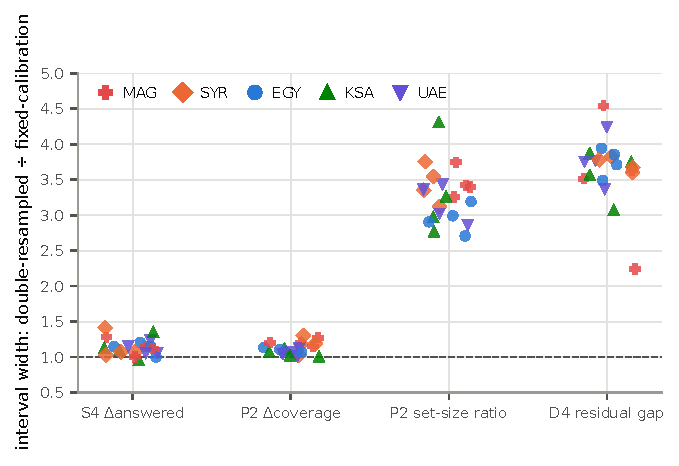
\includegraphics[width=0.74\textwidth]{figures/figC_interval_widths.pdf}
\caption{Width ratios: double-resampled interval divided by fixed-calibration interval for the stated quantities. Wider intervals reflect uncertainty in selecting the policy.}\label{fig:widths}
\end{figure}


% Allow the preceding robustness figure to float above the next page, while text fills this page.
\section{Model-assisted translation-equivalence screen}\label{model-assisted-screen}

GPT-6 Astra Extra High was used in separate sessions to screen 80 keys: 50 development keys (seed 20261104; 11 STEM, 13 humanities, 12 social sciences and 14 other) and 30 test keys (seed 20261106; 7, 8, 7 and 8 in those groups). The first session rated five MSA--dialect pairs per key, giving 400 pairs. A second session rated 150 pairs from 20 development and 10 test keys, and a third adjudicated those pairs. The protocol withheld model predictions and scores. The screening sample includes both development and test material; the sessions use one model and are not independent human raters.

Four checks allowed yes, no or unsure: Q1 asks whether meaning, conditions, quantities and terms are preserved; Q2 whether answer/options validity is preserved; Q3 whether the version is free of added hints or new ambiguity; Q4 whether the version belongs to the named dialect. The basic flag is Q1=no or Q2=no; the strict flag is any non-yes response in Q1--Q3. Thus the basic rate is composite and ``unsure'' is not equivalent to verified validity. Table~\ref{tab:auditflags} reproduces the first session's rates, with intervals clustered by question key. The screen intervals use 2,000 bootstrap replicates with seed 0 and lexicographically ordered keys. They replace the intervals from the original interactive analysis, whose seed was not recorded; rates and agreement estimates are unchanged. The accompanying text-free ratings and scripts reproduce these calculations and the association and sensitivity analyses below.

% Generated by tools/make_appendix_tables.py; do not edit data cells.
\begingroup
\setstretch{1}\small\setlength{\tabcolsep}{3pt}
\setlength{\LTleft}{0pt plus 1fill}\setlength{\LTright}{0pt plus 1fill}\setlength{\LTcapwidth}{\linewidth}
\setlength{\LTpre}{8pt}\setlength{\LTpost}{8pt}
\begin{longtable}{@{}>{\raggedright\arraybackslash}p{\dimexpr 0.0922000\linewidth-1.6000000\tabcolsep\relax}>{\raggedright\arraybackslash}p{\dimexpr 0.2269500\linewidth-1.6000000\tabcolsep\relax}>{\raggedright\arraybackslash}p{\dimexpr 0.2269500\linewidth-1.6000000\tabcolsep\relax}>{\raggedright\arraybackslash}p{\dimexpr 0.2269500\linewidth-1.6000000\tabcolsep\relax}>{\raggedright\arraybackslash}p{\dimexpr 0.2269500\linewidth-1.6000000\tabcolsep\relax}@{}}
\caption{Screen flag rates; model judgements rather than verified dataset defect rates.}\label{tab:auditflags}\\
\toprule
Var. & Basic flag & Q2 = no & Q3 = no & Strict flag \\
\midrule
\endfirsthead
\multicolumn{5}{l}{\small\itshape Table~\thetable\ (continued)}\\
\toprule
Var. & Basic flag & Q2 = no & Q3 = no & Strict flag \\
\midrule
\endhead
\midrule\endfoot
\bottomrule\endlastfoot
UAE & $0.44 [0.33, 0.55]$ & $0.06 [0.01, 0.12]$ & $0.41 [0.31, 0.53]$ & $0.60 [0.49, 0.70]$ \\*
EGY & $0.33 [0.23, 0.42]$ & $0.01 [0.00, 0.04]$ & $0.31 [0.21, 0.41]$ & $0.49 [0.38, 0.60]$ \\
KSA & $0.34 [0.24, 0.45]$ & $0.10 [0.04, 0.17]$ & $0.33 [0.23, 0.42]$ & $0.54 [0.42, 0.65]$ \\
SYR & $0.40 [0.29, 0.51]$ & $0.06 [0.01, 0.12]$ & $0.33 [0.23, 0.42]$ & $0.54 [0.42, 0.65]$ \\
MAG & $0.35 [0.25, 0.45]$ & $0.16 [0.09, 0.25]$ & $0.34 [0.24, 0.44]$ & $0.55 [0.44, 0.66]$ \\*
all & $0.37 [0.31, 0.43]$ & $0.08 [0.05, 0.11]$ & $0.34 [0.29, 0.40]$ & $0.54 [0.47, 0.62]$ \\
\end{longtable}
\endgroup


The basic flag rate is 0.32 [0.25, 0.40] on development keys and 0.45 [0.33, 0.57] on test keys. Q2 is unsure on 29\% of pairs, so the complement of its 8\% negative rate cannot be interpreted as confirmed validity. Sampling and criteria differ from the resource authors' human quality check.

Table~\ref{tab:auditagreement} reports agreement between the two screening sessions.

% Generated by tools/make_appendix_tables.py; do not edit data cells.
\begingroup
\setstretch{1}\small\setlength{\tabcolsep}{3pt}
\setlength{\LTleft}{0pt plus 1fill}\setlength{\LTright}{0pt plus 1fill}\setlength{\LTcapwidth}{\linewidth}
\setlength{\LTpre}{8pt}\setlength{\LTpost}{8pt}
\begin{longtable}{@{}>{\raggedright\arraybackslash}p{\dimexpr 0.3578900\linewidth-1.5000000\tabcolsep\relax}>{\raggedright\arraybackslash}p{\dimexpr 0.2947400\linewidth-1.5000000\tabcolsep\relax}>{\raggedright\arraybackslash}p{\dimexpr 0.1368400\linewidth-1.5000000\tabcolsep\relax}>{\raggedright\arraybackslash}p{\dimexpr 0.2105300\linewidth-1.5000000\tabcolsep\relax}@{}}
\caption{Within-model consistency across two sessions on 150 pairs. Cohen\textquotesingle s $\kappa$ uses three response categories.}\label{tab:auditagreement}\\
\toprule
Check & Observed agreement & $\kappa$ & Disagreements \\
\midrule
\endfirsthead
\multicolumn{4}{l}{\small\itshape Table~\thetable\ (continued)}\\
\toprule
Check & Observed agreement & $\kappa$ & Disagreements \\
\midrule
\endhead
\midrule\endfoot
\bottomrule\endlastfoot
Q1 meaning & $0.933$ & $0.86$ & $10$ \\*
Q2 answer/options & $0.707$ & $0.36$ & $44$ \\
Q3 clarity & $0.953$ & $0.90$ & $7$ \\*
Q4 dialect membership & $0.980$ & $0.00$ & $3$ \\
\end{longtable}
\endgroup


Q4 has $\kappa=0$ because one session assigned the same category to every double-rated pair, despite 98\% observed agreement. Q2 disagreement is mostly yes versus unsure. On the double-rated subset, basic flag rates are 0.34 in session one, 0.32 in session two and 0.33 after adjudication. Adjudication remains model-assisted rather than ground truth.

The association analysis contains 1,600 pair--model observations sharing 80 keys; they are not 1,600 independent items. Accuracy differences from MSA are $-4.5$ percentage points for unflagged pairs and $-6.2$ for basic-flagged pairs, with a flagged-minus-unflagged contrast of $-1.8$ [$-8.2$, $+5.1$] points. Answer-change rates are 26.9\% and 27.7\%, with contrast $+0.8$ [$-6.2$, $+7.9$] points. These intervals permit a material association and do not establish independence from translation validity.

Exclusions leave 45--54 keys per dialect. Mean answered-fraction differences remain negative ($-6$ to $-20$ points), but individual P1 estimates can change sign; Moroccan P1 interval widths range from 38 to 94 points. The full sensitivity CSV is supplied. Substituting MSA counterparts for flagged rows is a constructed scenario, not a clean dataset. The $f/(1-f)$ bound is uninformative here. Human equivalence labels remain unavailable.

\FloatBarrier
\section{Secondary and development analyses}\label{development-phase-experiments}

S1 (calibration efficiency) and S3 (calibration error) are secondary confirmatory analyses specified in the original plan. S1 uses 500 repeated subsamples of own-variety calibration keys at sizes 25, 50, 100, 150, 200, 250 and 400, then evaluates the nominal 0.70 set-coverage target on the fixed test set. Its within-target frequency is the fraction of these calibration subsamples yielding test coverage within 0.05 of 0.70. S3 reports mean confidence, expected calibration error with 15 equal-width bins, and multiclass Brier score \cite{guo2017calibration}. Tables~\ref{tab:s1} and~\ref{tab:s3} summarise these results; full outputs are provided in the supplementary CSV files.

% Generated by tools/make_appendix_tables.py; do not edit data cells.
\begingroup
\setstretch{1}\small\setlength{\tabcolsep}{3pt}
\setlength{\LTleft}{0pt plus 1fill}\setlength{\LTright}{0pt plus 1fill}\setlength{\LTcapwidth}{\linewidth}
\setlength{\LTpre}{8pt}\setlength{\LTpost}{8pt}
\begin{longtable}{@{}>{\raggedright\arraybackslash}p{\dimexpr 0.2381000\linewidth-1.3333333\tabcolsep\relax}>{\raggedright\arraybackslash}p{\dimexpr 0.4047600\linewidth-1.3333333\tabcolsep\relax}>{\raggedright\arraybackslash}p{\dimexpr 0.3571400\linewidth-1.3333333\tabcolsep\relax}@{}}
\caption{S1 ranges over the 20 dialect--model cells: empirical frequency of coverage within 0.05 of 0.70, and mean achieved coverage. These ranges are not confidence intervals.}\label{tab:s1}\\
\toprule
Calibration keys & Within-target frequency & Mean coverage \\
\midrule
\endfirsthead
\multicolumn{3}{l}{\small\itshape Table~\thetable\ (continued)}\\
\toprule
Calibration keys & Within-target frequency & Mean coverage \\
\midrule
\endhead
\midrule\endfoot
\bottomrule\endlastfoot
25 & $0.312\text{--}0.488$ & $0.701\text{--}0.747$ \\*
50 & $0.460\text{--}0.672$ & $0.674\text{--}0.722$ \\
100 & $0.522\text{--}0.850$ & $0.668\text{--}0.722$ \\
150 & $0.634\text{--}0.928$ & $0.668\text{--}0.724$ \\
200 & $0.676\text{--}0.980$ & $0.666\text{--}0.723$ \\
250 & $0.652\text{--}0.992$ & $0.660\text{--}0.722$ \\*
400 & $0.730\text{--}1.000$ & $0.660\text{--}0.721$ \\
\end{longtable}
\endgroup


% Generated by tools/make_appendix_tables.py; do not edit data cells.
\begingroup
\setstretch{1}\small\setlength{\tabcolsep}{3pt}
\setlength{\LTleft}{0pt plus 1fill}\setlength{\LTright}{0pt plus 1fill}\setlength{\LTcapwidth}{\linewidth}
\setlength{\LTpre}{8pt}\setlength{\LTpost}{8pt}
\begin{longtable}{@{}>{\raggedright\arraybackslash}p{\dimexpr 0.1428571\linewidth-1.6000000\tabcolsep\relax}>{\raggedright\arraybackslash}p{\dimexpr 0.2142857\linewidth-1.6000000\tabcolsep\relax}>{\raggedright\arraybackslash}p{\dimexpr 0.2142857\linewidth-1.6000000\tabcolsep\relax}>{\raggedright\arraybackslash}p{\dimexpr 0.2142857\linewidth-1.6000000\tabcolsep\relax}>{\raggedright\arraybackslash}p{\dimexpr 0.2142857\linewidth-1.6000000\tabcolsep\relax}@{}}
\caption{S3: expected calibration error / multiclass Brier score on the confirmatory test. Full confidence and Brier intervals are in the CSV.}\label{tab:s3}\\
\toprule
Var. & ALLaM & Fanar & Qwen3 & Gemma \\
\midrule
\endfirsthead
\multicolumn{5}{l}{\small\itshape Table~\thetable\ (continued)}\\
\toprule
Var. & ALLaM & Fanar & Qwen3 & Gemma \\
\midrule
\endhead
\midrule\endfoot
\bottomrule\endlastfoot
MSA & $0.174\,/\,0.563$ & $0.049\,/\,0.480$ & $0.046\,/\,0.467$ & $0.052\,/\,0.520$ \\*
MAG & $0.219\,/\,0.676$ & $0.037\,/\,0.565$ & $0.045\,/\,0.583$ & $0.055\,/\,0.599$ \\
SYR & $0.213\,/\,0.662$ & $0.041\,/\,0.560$ & $0.035\,/\,0.541$ & $0.045\,/\,0.601$ \\
EGY & $0.205\,/\,0.622$ & $0.029\,/\,0.530$ & $0.033\,/\,0.508$ & $0.050\,/\,0.567$ \\
KSA & $0.206\,/\,0.628$ & $0.038\,/\,0.525$ & $0.052\,/\,0.506$ & $0.054\,/\,0.564$ \\
UAE & $0.213\,/\,0.620$ & $0.044\,/\,0.513$ & $0.042\,/\,0.501$ & $0.064\,/\,0.548$ \\*
ENG & $0.168\,/\,0.505$ & $0.036\,/\,0.376$ & $0.073\,/\,0.322$ & $0.040\,/\,0.381$ \\
\end{longtable}
\endgroup


Development experiments examined hidden-state variety routing, correctness probes and a mean-direction representation intervention. The log reports no consistent advantage that supported replacing the text router with an internal router, and no supported recovery from the representation intervention. Some early internal measurements required implementation corrections. These observations informed development but did not establish a mechanism for the confirmatory gaps; the historical development excerpt is included with the supplementary documentation.

\FloatBarrier
\begin{adjustwidth}{-\extralength}{0cm}
\reftitle{References}
\bibliography{references}
\PublishersNote{}
\end{adjustwidth}
\end{document}
